
\documentclass[conference]{IEEEtran}

\usepackage{float} 
\usepackage{url}  
\usepackage{multirow}
\usepackage{caption}
\usepackage{subcaption}
\usepackage{booktabs}
\usepackage{cite}
\pagestyle{plain}
\usepackage{amsmath}
\usepackage{float}
\usepackage{tikz}
\usetikzlibrary{shapes.geometric, arrows, positioning}
\usepackage{placeins}
\usepackage{comment}
\usepackage{tabularx}
\ifCLASSINFOpdf
  \usepackage[pdftex]{graphicx}
\fi

\hyphenation{op-tical net-works semi-conduc-tor}

\begin{document}


\title{Lacuna Solar Survey Challenge: Counting Photovoltaic and Solar Panels from Aerial Imagery}

\author{\IEEEauthorblockN{\\ Hugo Veríssimo}
\IEEEauthorblockA{Complements of Machine Learning 24/25\\
University of Aveiro\\
Aveiro, Portugal\\
hugoverissimo@ua.pt}
\and
\IEEEauthorblockN{\\ João Cardoso}
\IEEEauthorblockA{Complements of Machine Learning 24/25\\
University of Aveiro\\
Aveiro, Portugal\\
joaopcardoso@ua.pt}}

\maketitle
\thispagestyle{plain}

\begin{abstract}
This project was developed with the Lacuna Solar Survey Challenge in mind, to create a model capable of identifying photovoltaic and thermal solar panels from aerial imagery (satellite or drone). The challenge is of public interest, to learn about solar panel usage, and support in planning infrastructure in Madagascar. The dataset presented issues such as inconsistent masks and a severe class imbalance, which required manual curation. Three types of models were developed: a hybrid approach, of image-based regression combined with metadata based estimation, object detection, and instance segmentation, where the former was the best performing model. The benchmark results indicated that there remains room for improvement, which would necessitate a more refined curation of the dataset as well as increased computational resources.
\end{abstract}

\begin{quote}
\small
\noindent
\textbf{Keywords:} solar panel detection, deep learning, image feature extraction, object detection, instance segmentation
%Zindi challenge, aerial imagery,
\end{quote}

\IEEEpeerreviewmaketitle


\section{Introduction}

Access to electricity and hot water has been a basic necessity for a long time in the developed world. In developing countries, the lack of a centralized distribution system makes this access harder for everyone. To address this gap, it is essential for governments, non-governmental organizations, and energy suppliers to understand how solar photovoltaic and solar thermal panels (for electricity and water heating, respectively) are distributed throughout the territory to ensure proper planning and effective policy making. In this context, a challenge was created by the Lacuna Fund and associate entities in the Zindi platform to develop a machine learning model capable of accurately counting the number of solar thermal and photovoltaic panels in drone and satellite imagery.

In the present work, we have developed different approaches to the problem at hand, where we need to count the two types of panels separately: taking a regression type approach, where images are analysed as a whole and the target number of panels are provided per image; by identifying the panels through object detection and counting them afterwards; and by applying segmentation models to identify the regions of interest, analysing them and counting the panels. The different approaches were developed so that a single model for each type would be able to tackle the task of identifying and counting the different panels.

\section{State of The Art}

The task of detection of solar panels serves many purposes, with the strongest focus of the works here documented being on the detection and localization of solar panels in large areas (countries). This type of assessment allows for proper planning of infrastructure, and to adapt current maintenance through peak output of dense areas with solar panels.

In the work of Malof \textit{et al.} (2016) the authors developed an automatic detection model of solar arrays, specific for photovoltaic panels. The model developed had computational efficiency at the forefront, with the purpose of being deployed nation wide in the United States, hence a multi-stage approach consisting of: pixel-wise feature extraction; Random Forest (RF) Classifier; post-processing to improve the pixel-wise classification accuracy for the object detection phase; finalizing with the object detection, via thresholding the finalized confidence map. This algorithm presents superior performance to standalone RF, and was well remarked as an initial assessment methodology for large areas \cite{Malof_2016}. 

The \textit{DeepSolar} model allowed the creation of a nearly complete contiguous solar panel installation map, and consists of two parts, with different purposes: first, via transfer learning, the convolutional neural network (CNN) classifier is trained on labelled imagery that merely indicates the presence or absence of panels (though the volume of data is considerable, at almost 400 000 images just for this task). The model is then enhanced by adding an additional CNN branch directly connected to the intermediate layers to add segmentation capabilities to the model. The difference is that this approach allows the model to be trained on the same dataset and to "greedily" extract the relevant features associated with solar panels, learning in a semi-supervised manner. The model was able to achieve the best result of 93.7\% precision and 90.5\% recall in non-residential areas \cite{Yu2018DeepSolar}.

Different models have been proposed for panel detection through image segmentation, using Mask R-CNN \cite{maskrcnn} , TernausNet, based on U-Net \cite{KAUSIKA2021100111}, MobileNet with U-Net backbone \cite{wani2021segmentation}, with different approaches to data preparation and application. These models consistently score higher than 90\% in terms of precision, at the cost of higher computation times compared to the examples previously mentioned (also for very different task sizes). A couple notable aspects across publications: the size of datasets (often in the tens of thousands of images), with strong strategies for collecting and/or preprocessing, ensuring that the models have the best possible starting point to learn and develop; and the focus on a specific type of panel or problem topic, not trying to solve multiple problems with a single tool.

For the purpose of this work, three approaches to the problem were developed to assess their strengths and merits, which will be detailed in the following subsections.

\subsection{Image-based Regression}

Considering that each image is labelled in terms of amount of photovoltaic and thermal solar panels, the conditions for training considering a regression approach are available. For this, deep neural networks (convolutional neural networks, CNN) were considered for their excellent capabilities in extracting spatial features, but each with a distinguishing feature.

ResNet (Residual Networks) was introduced in 2015 by Microsoft, and is notorious for dealing with vanishing gradient problem by skipping connections between neuron layers \cite{ResNet}. This allows the model to grow and have several layers (over 100), making it capable of learning a larger variety of features from the first to the deeper layers, without suffering from performance degradation.

DenseNet follows on the footsteps of ResNet, and was introduced in 2016 by Huang \textit{et al.}, whereby the idea of skipping connections is taken further, and every layer prior to a given layer is connected to it \cite{DenseNet}. This avoids the chain multiplication problem (which leads to vanishing gradients), while reusing previously learned features, retaining relevant information throughout the deepness of the CNN. This architecture also has the benefit of using less parameters than CNN in general (and ResNet as well).

EfficientNet (EffNet), the most recent of this group was introduced by Google AI in 2019, and departs from the direct implementation of the aforementioned methods, dealing with vanishing gradients given its intrinsic architecture \cite{EffienctNet}. By having MBConv (Mobile Inverted Bottleneck Convolution) as its building block, it allows to extract spatial features by expanding the number of channels to perform depthwise convolution and applying separate filters per channel, that is then compressed to the original size of the input. Whilst this happens, the mechanism of squeeze-and-excitation determines the importance of said features, further addressing the vanishing gradient problem. This architecture is then scaled via compound scaling (rather than arbitrarily), whereby the size of the CNN (input resolution, depth and width) is scaled in a balanced manner, with the compound coefficient $\phi$ being adjusted by grid search.

\subsection{Object Detection}

With object detection, the model is trained on the basis of bounding boxes surrounding the subject of interest, in order to be able to identify them in new environments and types of image. With multiple classes, the model discerns between labels with class probabilities, estimated from the extracted features of the assessed boxes (using a CNN) throughout the image. One of the most famous and used models is YOLO ("You Only Look Once") introduced in 2015 by Redmon \& Fardhi, being a crucial model in fast object detection and localization \cite{YOLO}. In a single stage, the model addresses the localization and detection problems, where a CNN backbone (that has changed with the released versions) is used, with feature fusion layers (akin to the way learned features are reused, involving various algorithms), and an output of the likelihood of a class and the location of the bounding boxes.

\subsection{Instance Segmentation}

Building on the concepts presented previously on object detection, instance segmentation addresses the problem of identification by incorporating the information of object masks \cite{YOLOSeg}. These are tighter around the object (than bounding boxes), which serve to add a layer to the YOLO algorithm. A global prototype mask (that works with a separate, smaller CNN) is generated for the whole image - this way once the bounding box is determined, mask coefficients are estimated in order to combine the prototype masks into an instance-specific mask. This approach avoids per mask full resolution segmentation, keeping the model size small and fast.



\section{Methodology}

\subsection{Dataset \& EDA}

The dataset was provided within the Zindi challenge \cite{zindi2025lacuna}, consisting of 4419 images, and per image metadata, consisting of the source (drone or satellite), mask placement, and context of the installation surroundings (e.g., roof, floor, array).

Of all the images, 3312 (75\%) have detailed information on the masks (location, number of panels within, if they are photovoltaic or thermal). The remaining 1107 (25\%) do not have this information, only the metadata related to the image. Hence, per design of the competition the train/test split is 75/25.

\begin{figure}[H]
    \centering
    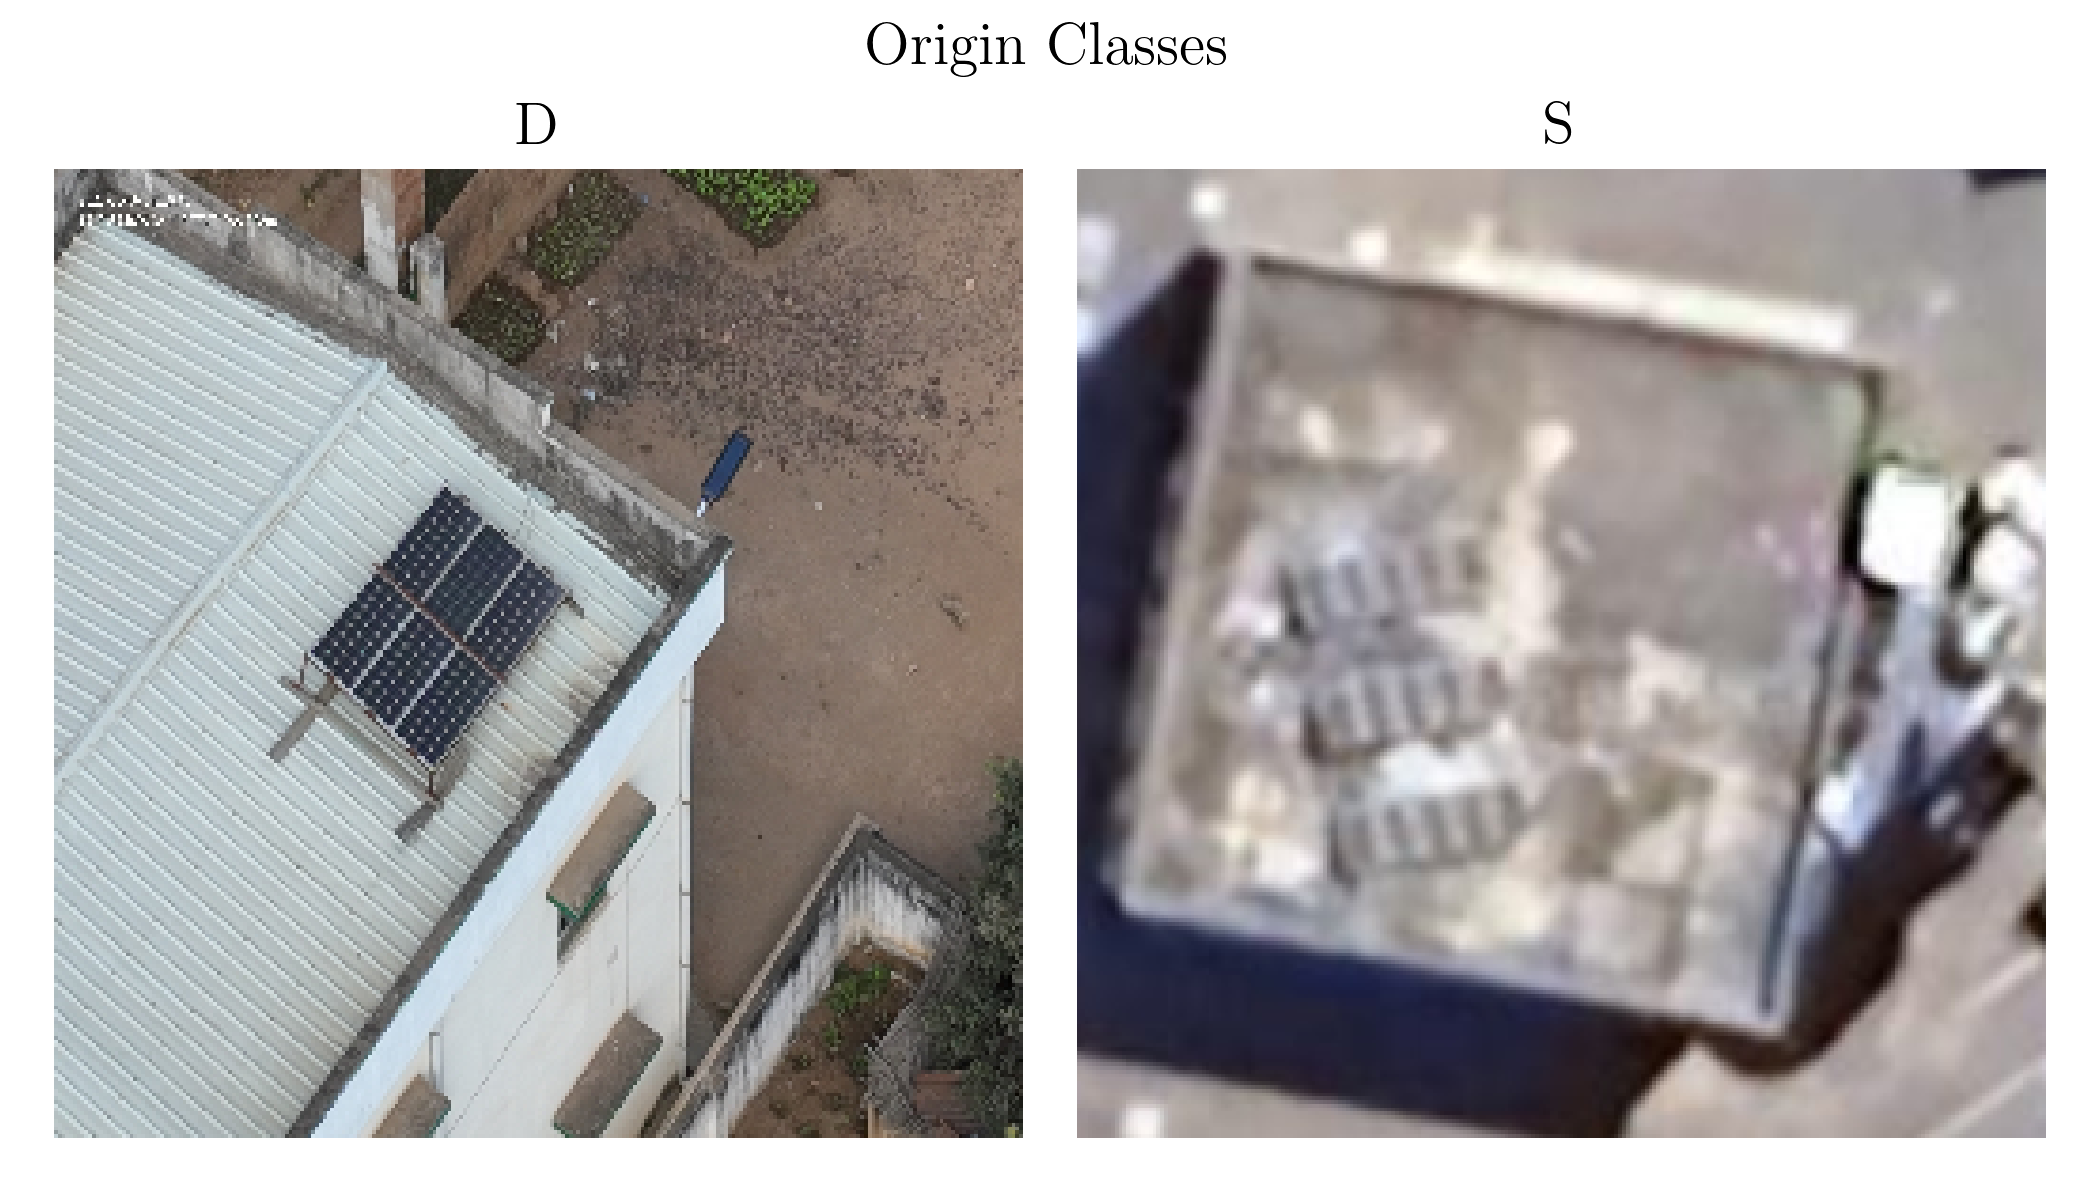
\includegraphics[width=1\linewidth]{assets/data_origin_classes.png}
    \caption{Images of photovoltaic panels placed on the roof, from drone (left side) and satellite (right side). The difference in resolution between them is evident.}
    \label{fig:data_origin_classes}
\end{figure}

\begin{figure}[H]
    \centering
    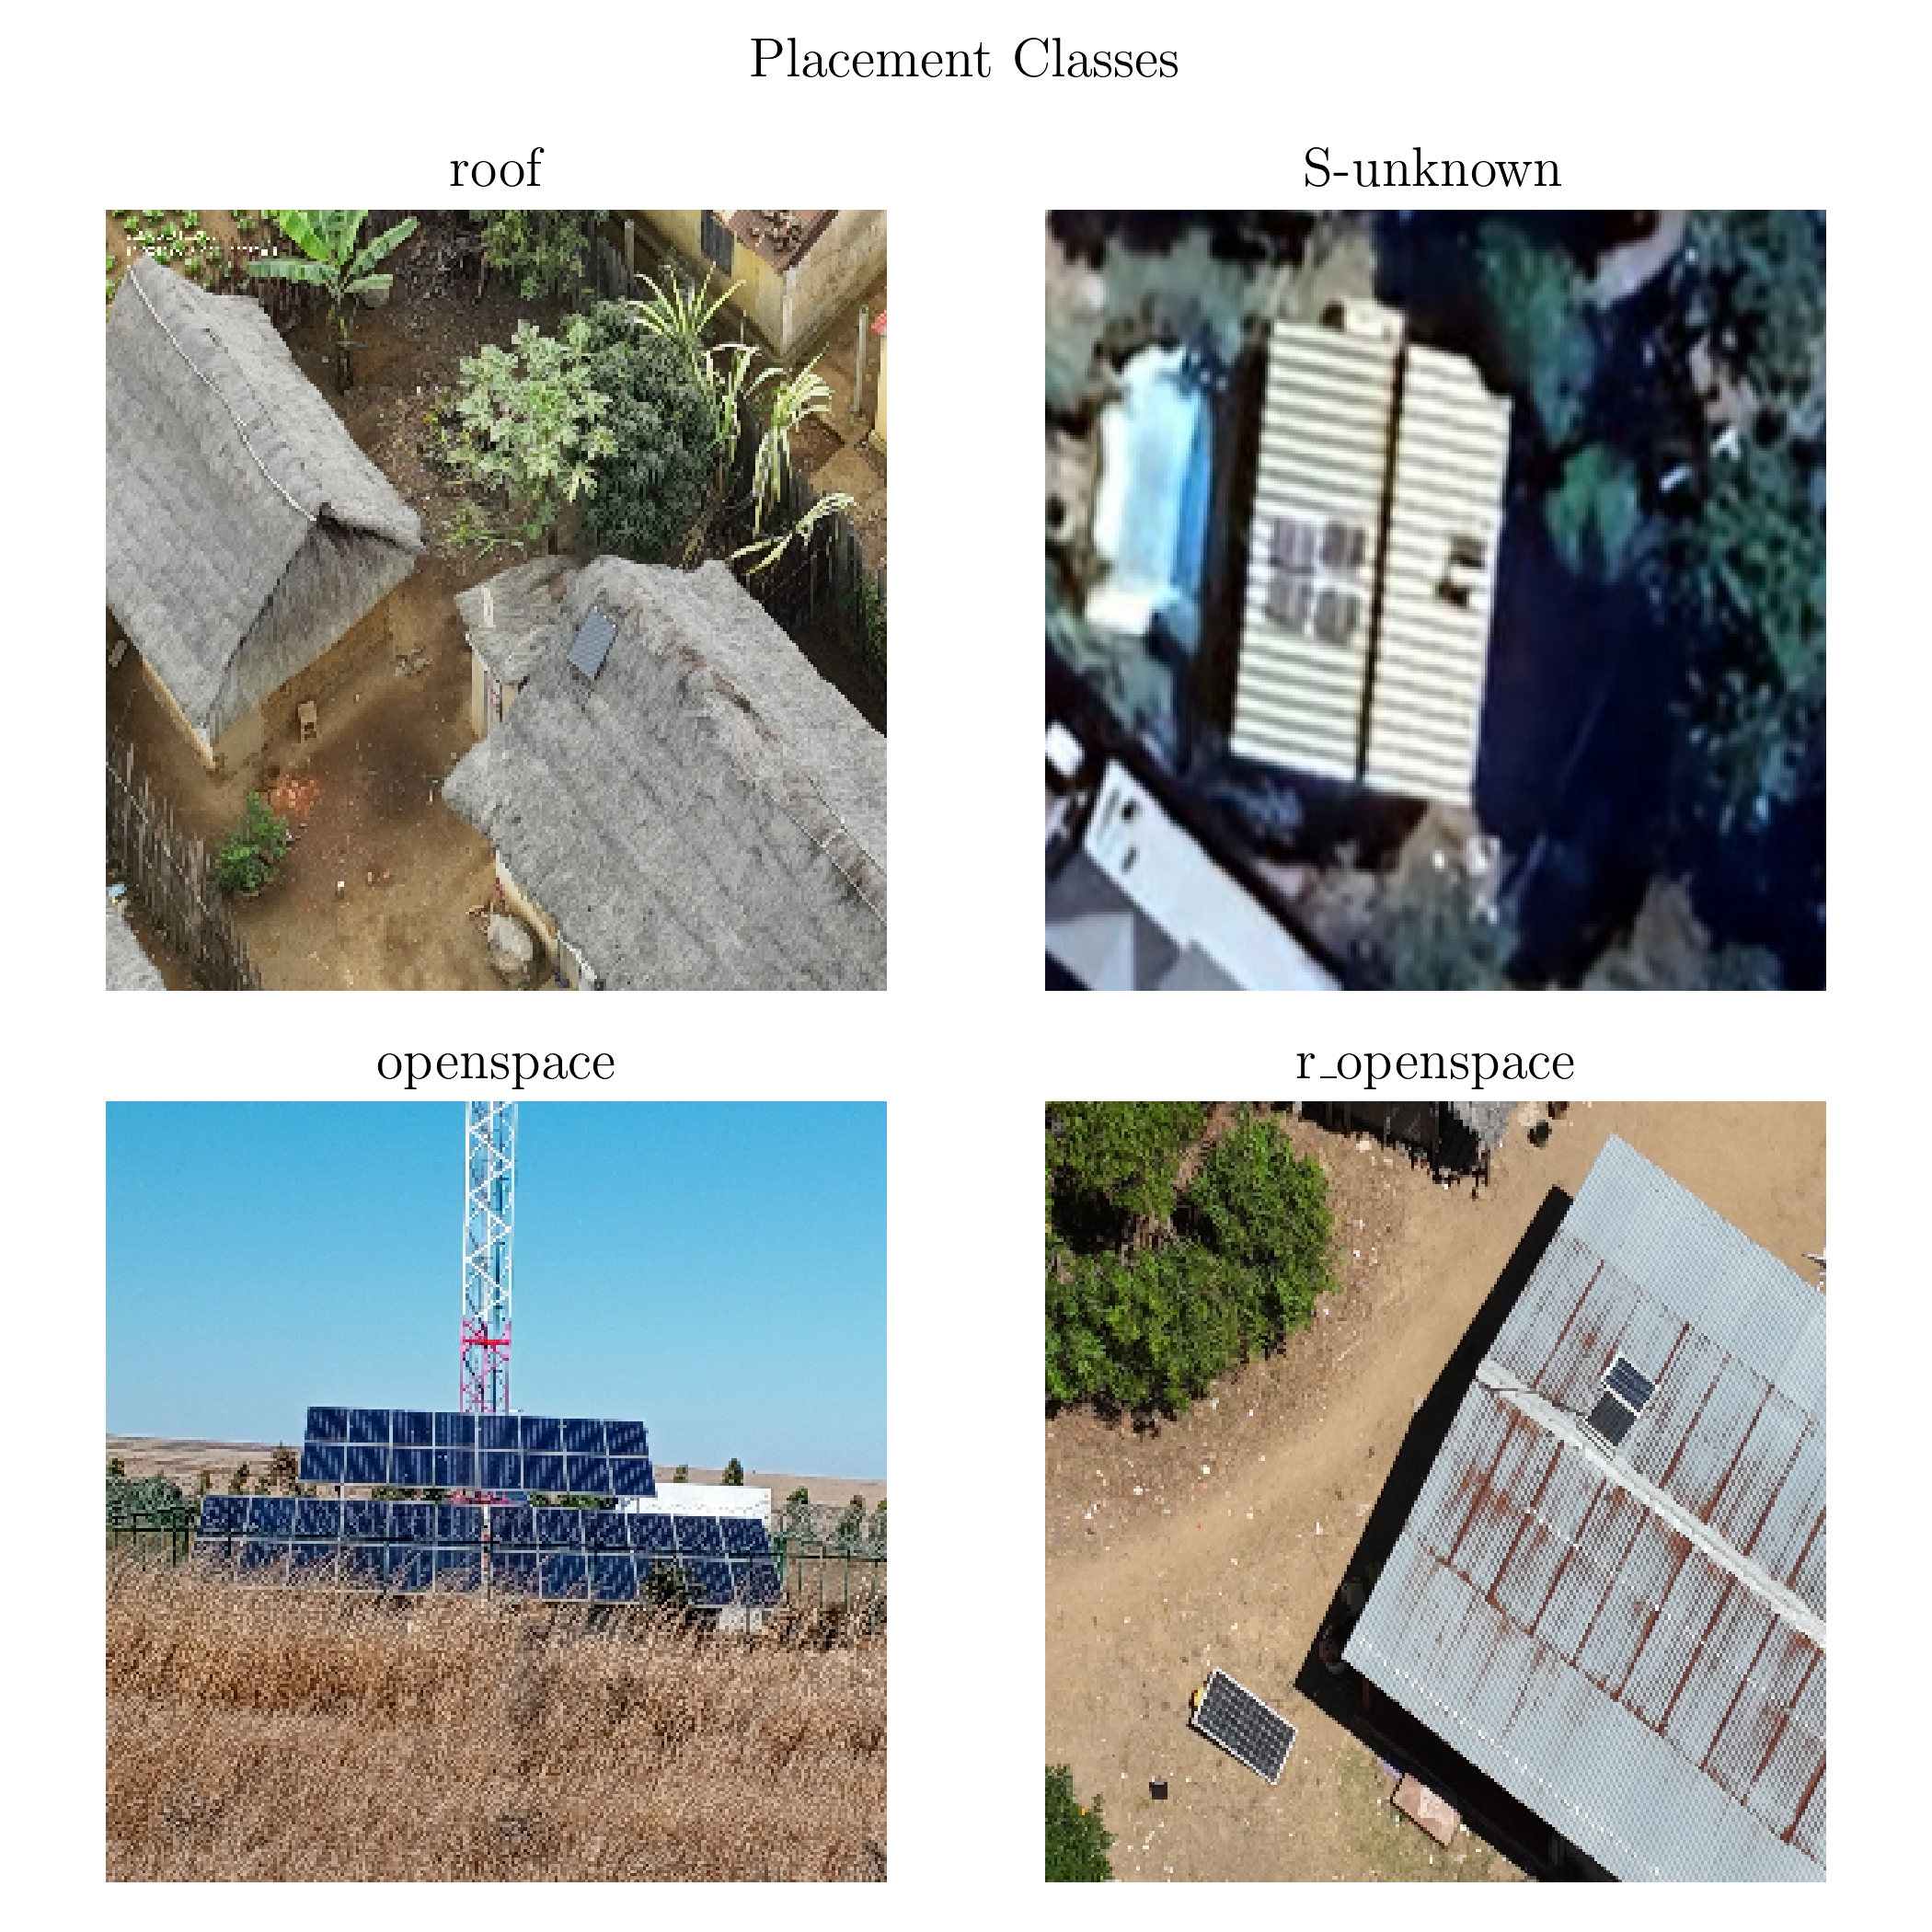
\includegraphics[width=1\linewidth]{assets/data_placement_classes.png}
    \caption{The different panel placement possibilities (top right is from satellite imagery). Bottom left image shows an image that is atypical for a drone style image.}
    \label{fig:data_placement_classes}
\end{figure}

In Fig. \ref{fig:data_placement_classes} the image origin and placement are displayed, which according to the challenge information were labelled by expert personnel. Where the placement class was inconclusive, the images are labelled as "S-unknown" (the remaining examples are self-explanatory). Besides the two classes to be identified, the context and origin of the images means a considerable number of combinations for the model to learn, where some of these combinations might (and certainly are), under-represented given the relatively small dataset.

The masks are not consistent throughout the dataset, with a varying number of panels within them (some contain a single panel, others might contain a complete array of up to 200), which can be clearly seen in Fig. \ref{fig:data_objectdistribution}. In addition to this inconsistency, there is also a strong imbalance between photovoltaic and solar thermal panels, with approximately 95\% of the dataset corresponding to photovoltaic panels.

From the sample images below, the difference in the quality of the masks is stark. Several images were found to have misaligned vertices of the masks, and several masks had a large number of panels (as seen from the distribution aforementioned). In principle, with the reference of the number of panels within each mask, it might have a small impact on some types of models, but the same model is in fact learning features for different representations: rather than for the representation of individual panels. This was an evident obstacle to the implementation of YOLO type models, which was dealt with, and further detailed in the following sections.

\begin{figure}[H]
    \centering
    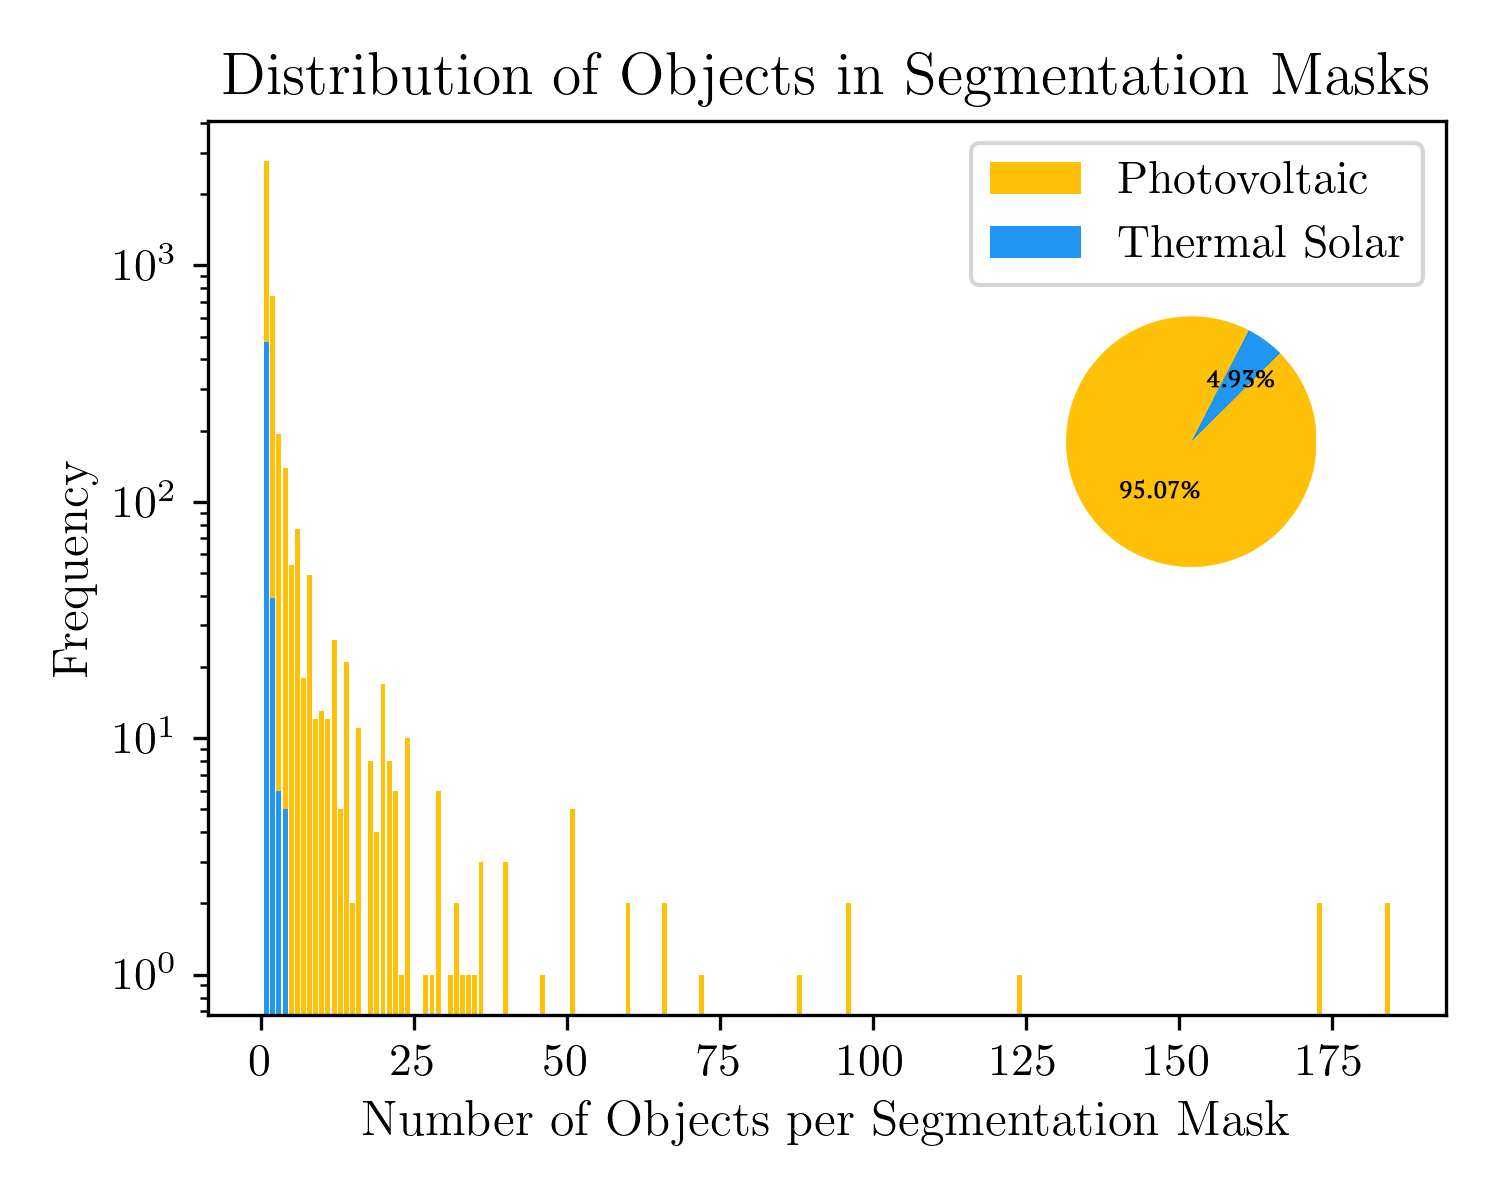
\includegraphics[width=1\linewidth]{assets/data_objectdistribution_ph.png}
    \caption{Distribution of the number of panels within a single mask.}
    \label{fig:data_objectdistribution}
\end{figure}

% REVER HUGO: legenda da figura está incorrecta (usar igual ao que está na Fig. 3)
\begin{figure}[H]
    \centering
    \begin{subfigure}[b]{\linewidth}
        \centering
        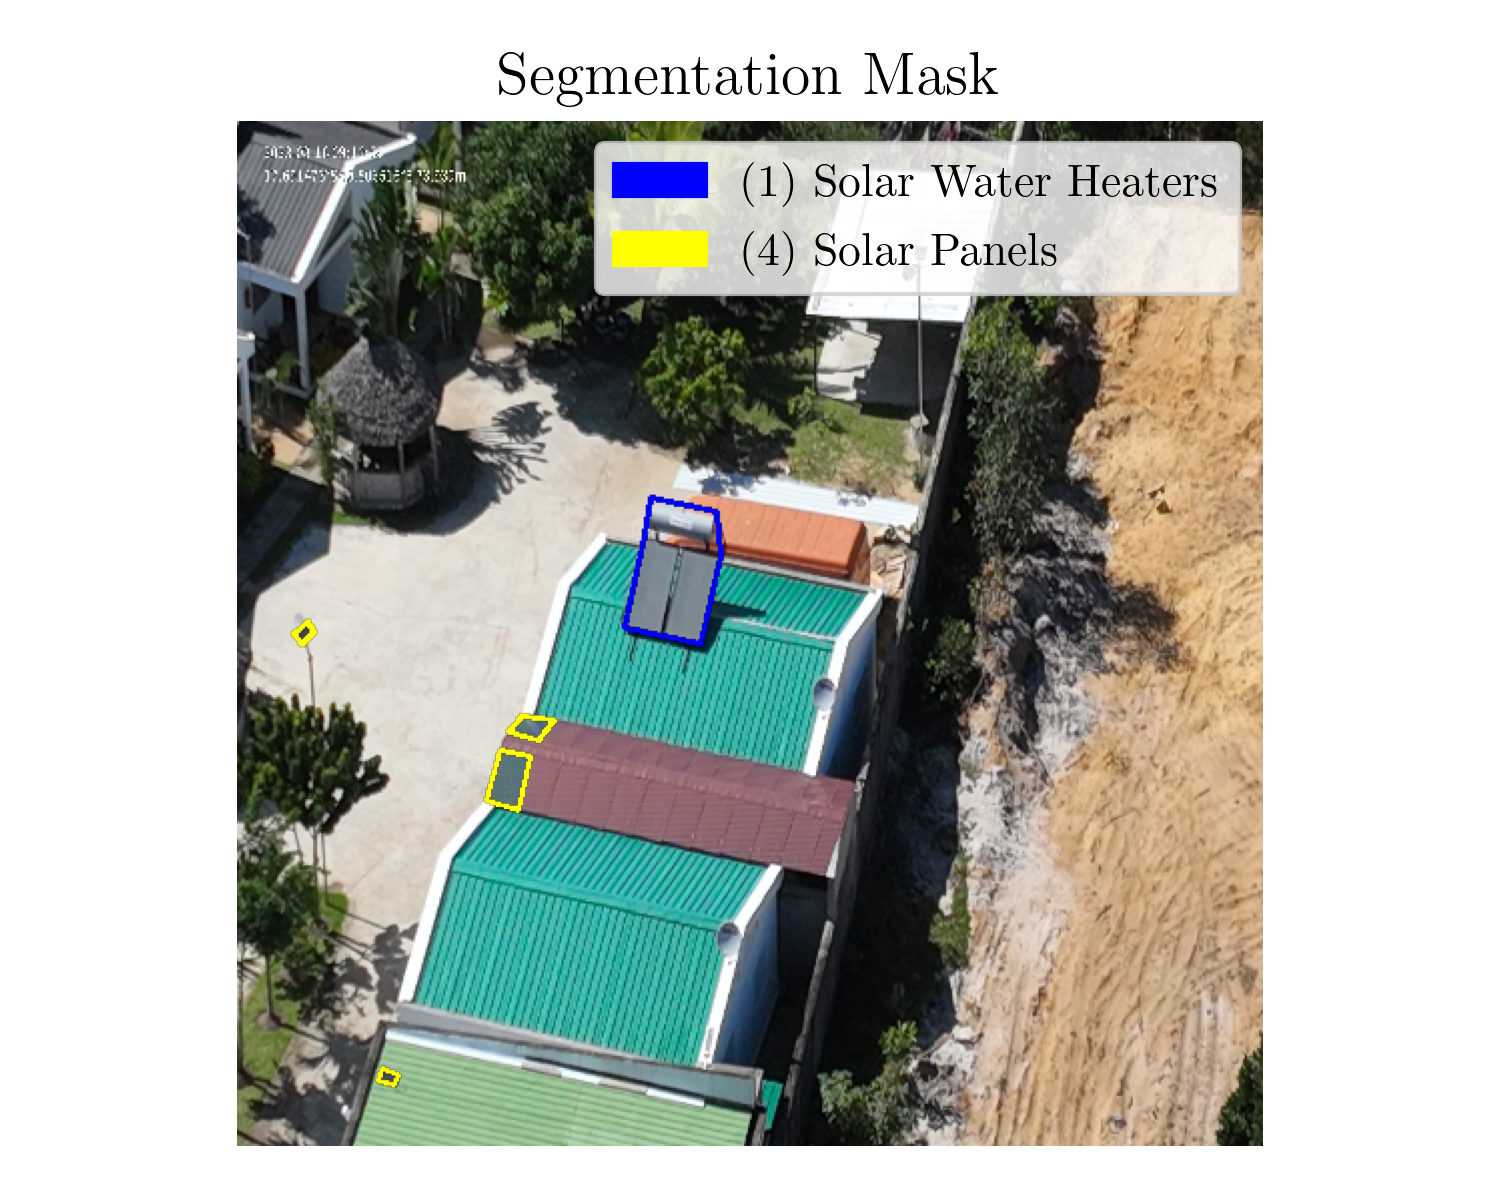
\includegraphics[width=\linewidth]{assets/data_segmentation_mask.png}
        \caption{Sample image of accurate labelling, with a single panel per mask.}
        \label{fig:data_segmentation_mask}
    \end{subfigure}

    \begin{subfigure}[b]{\linewidth}
        \centering
        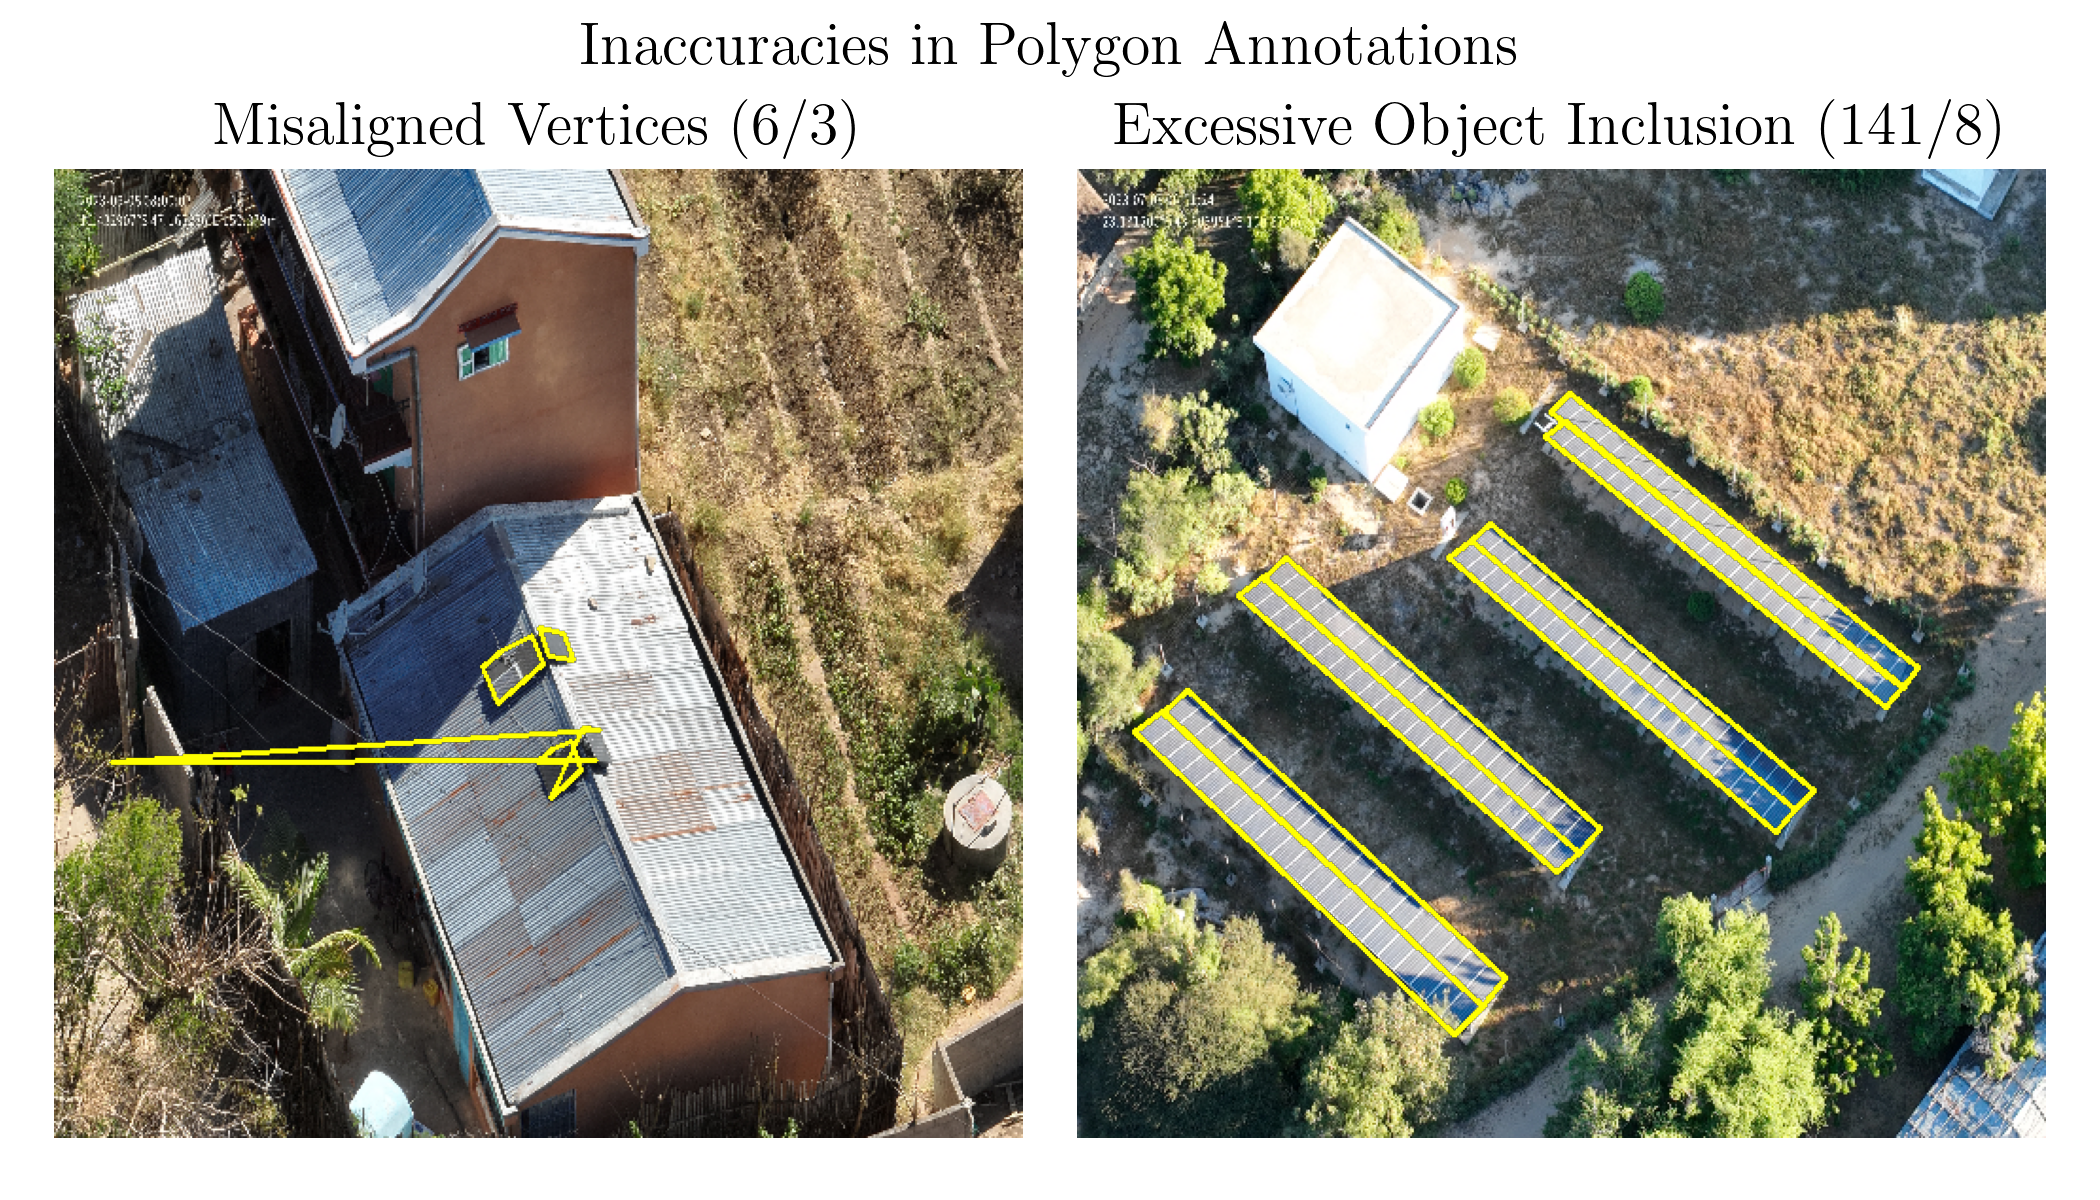
\includegraphics[width=\linewidth]{assets/data_poly_problems.png}
        \caption{Sample images of incorrectly marked masks: (on the left) mask distorted, misrepresenting the panel; (on the right) excessive objects within a single mask.}
        \label{fig:data_poly_problems}
    \end{subfigure}
    \caption{Sample images from the Zindi dataset.}
    \label{fig:combined_segmentation_poly_issues}
\end{figure}


\subsection{Preprocessing}

The discussion forum for the competition was a fruitful source of information on the dataset and how to address it. As seen before, the incorrectly defined masks, and the masks with several panels represented hindrances to achieve the best possible performance. Besides that, some of the masks were shifted from the actual position of the panels, which considering that all were identically shifted, seemed deliberate from the competition. By manually analysing every image  it was possible to detect such images (with wrongly drawn masks and shifted), and correct them. Upon completing the dataset revision, 263 of the training samples were discarded due to poorly drawn masks (the remaining images that had misaligned masks were corrected).

Once the dataset was ready, an online data augmentation process was devised in order to increase the amount of training data and diversify it, enhancing the generalizability of the trained models. The transformations HorizontalFlip, VerticalFlip, RandomRotate90, GaussianBlur, CLAHE (Contrast Limited Adaptive Histogram Equalization), HueSaturationValue and Normalize were applied before all training cycles. The images were all resized to 512x512, to lower the computational burden and homogenize the code throughout the pipeline. 

\section{Models}

In the following subsections, A through C, the approach and results of the developed models are presented. The hybrid model \textit{zulo40} is used as a benchmark, as it was one of the best-performing in the competition and was kindly shared in the discussion forum. The models in subsection \textit{A. Image-based Regression} are based on this model's approach. The models in \textit{A. Image-based Regression} were selected from PyTorch (\texttt{torchvision}) package, and the ones from \textit{B. Object Detection} and \textit{C. Instance Segmentation} are from \texttt{ultralytics} package.
%verificar formatação do texto a mencionar os packages, e usar igual
% JP: Pequenas correções de palavras

The training examples were split between training and validation (80/20) across all the models' training. The best set of hyperparameters was selected from a randomized search in a cross-validation (CV) set up. Unlike what is commonly done with K-fold CV, due to the long processing times and high computational load, the number of CV repetitions was adjusted 3 times (and not the usual 5 times), and averaged over them. We acknowledge the downside of this approach, particularly the fact that only 60\% of the data is exposed to validation and the reduced diversity of the models trained. These aspects become particularly evident due to the relatively small size of the dataset.

\subsection{Image-based Regression}

This approach had the purpose of incorporating the information from the metadata in the labels with the feature extracted with CNN backbone by transfer learning. In Fig. \ref{fig:nn} we present the schematics for the model's architecture.

\begin{figure}[H]
    \centering
    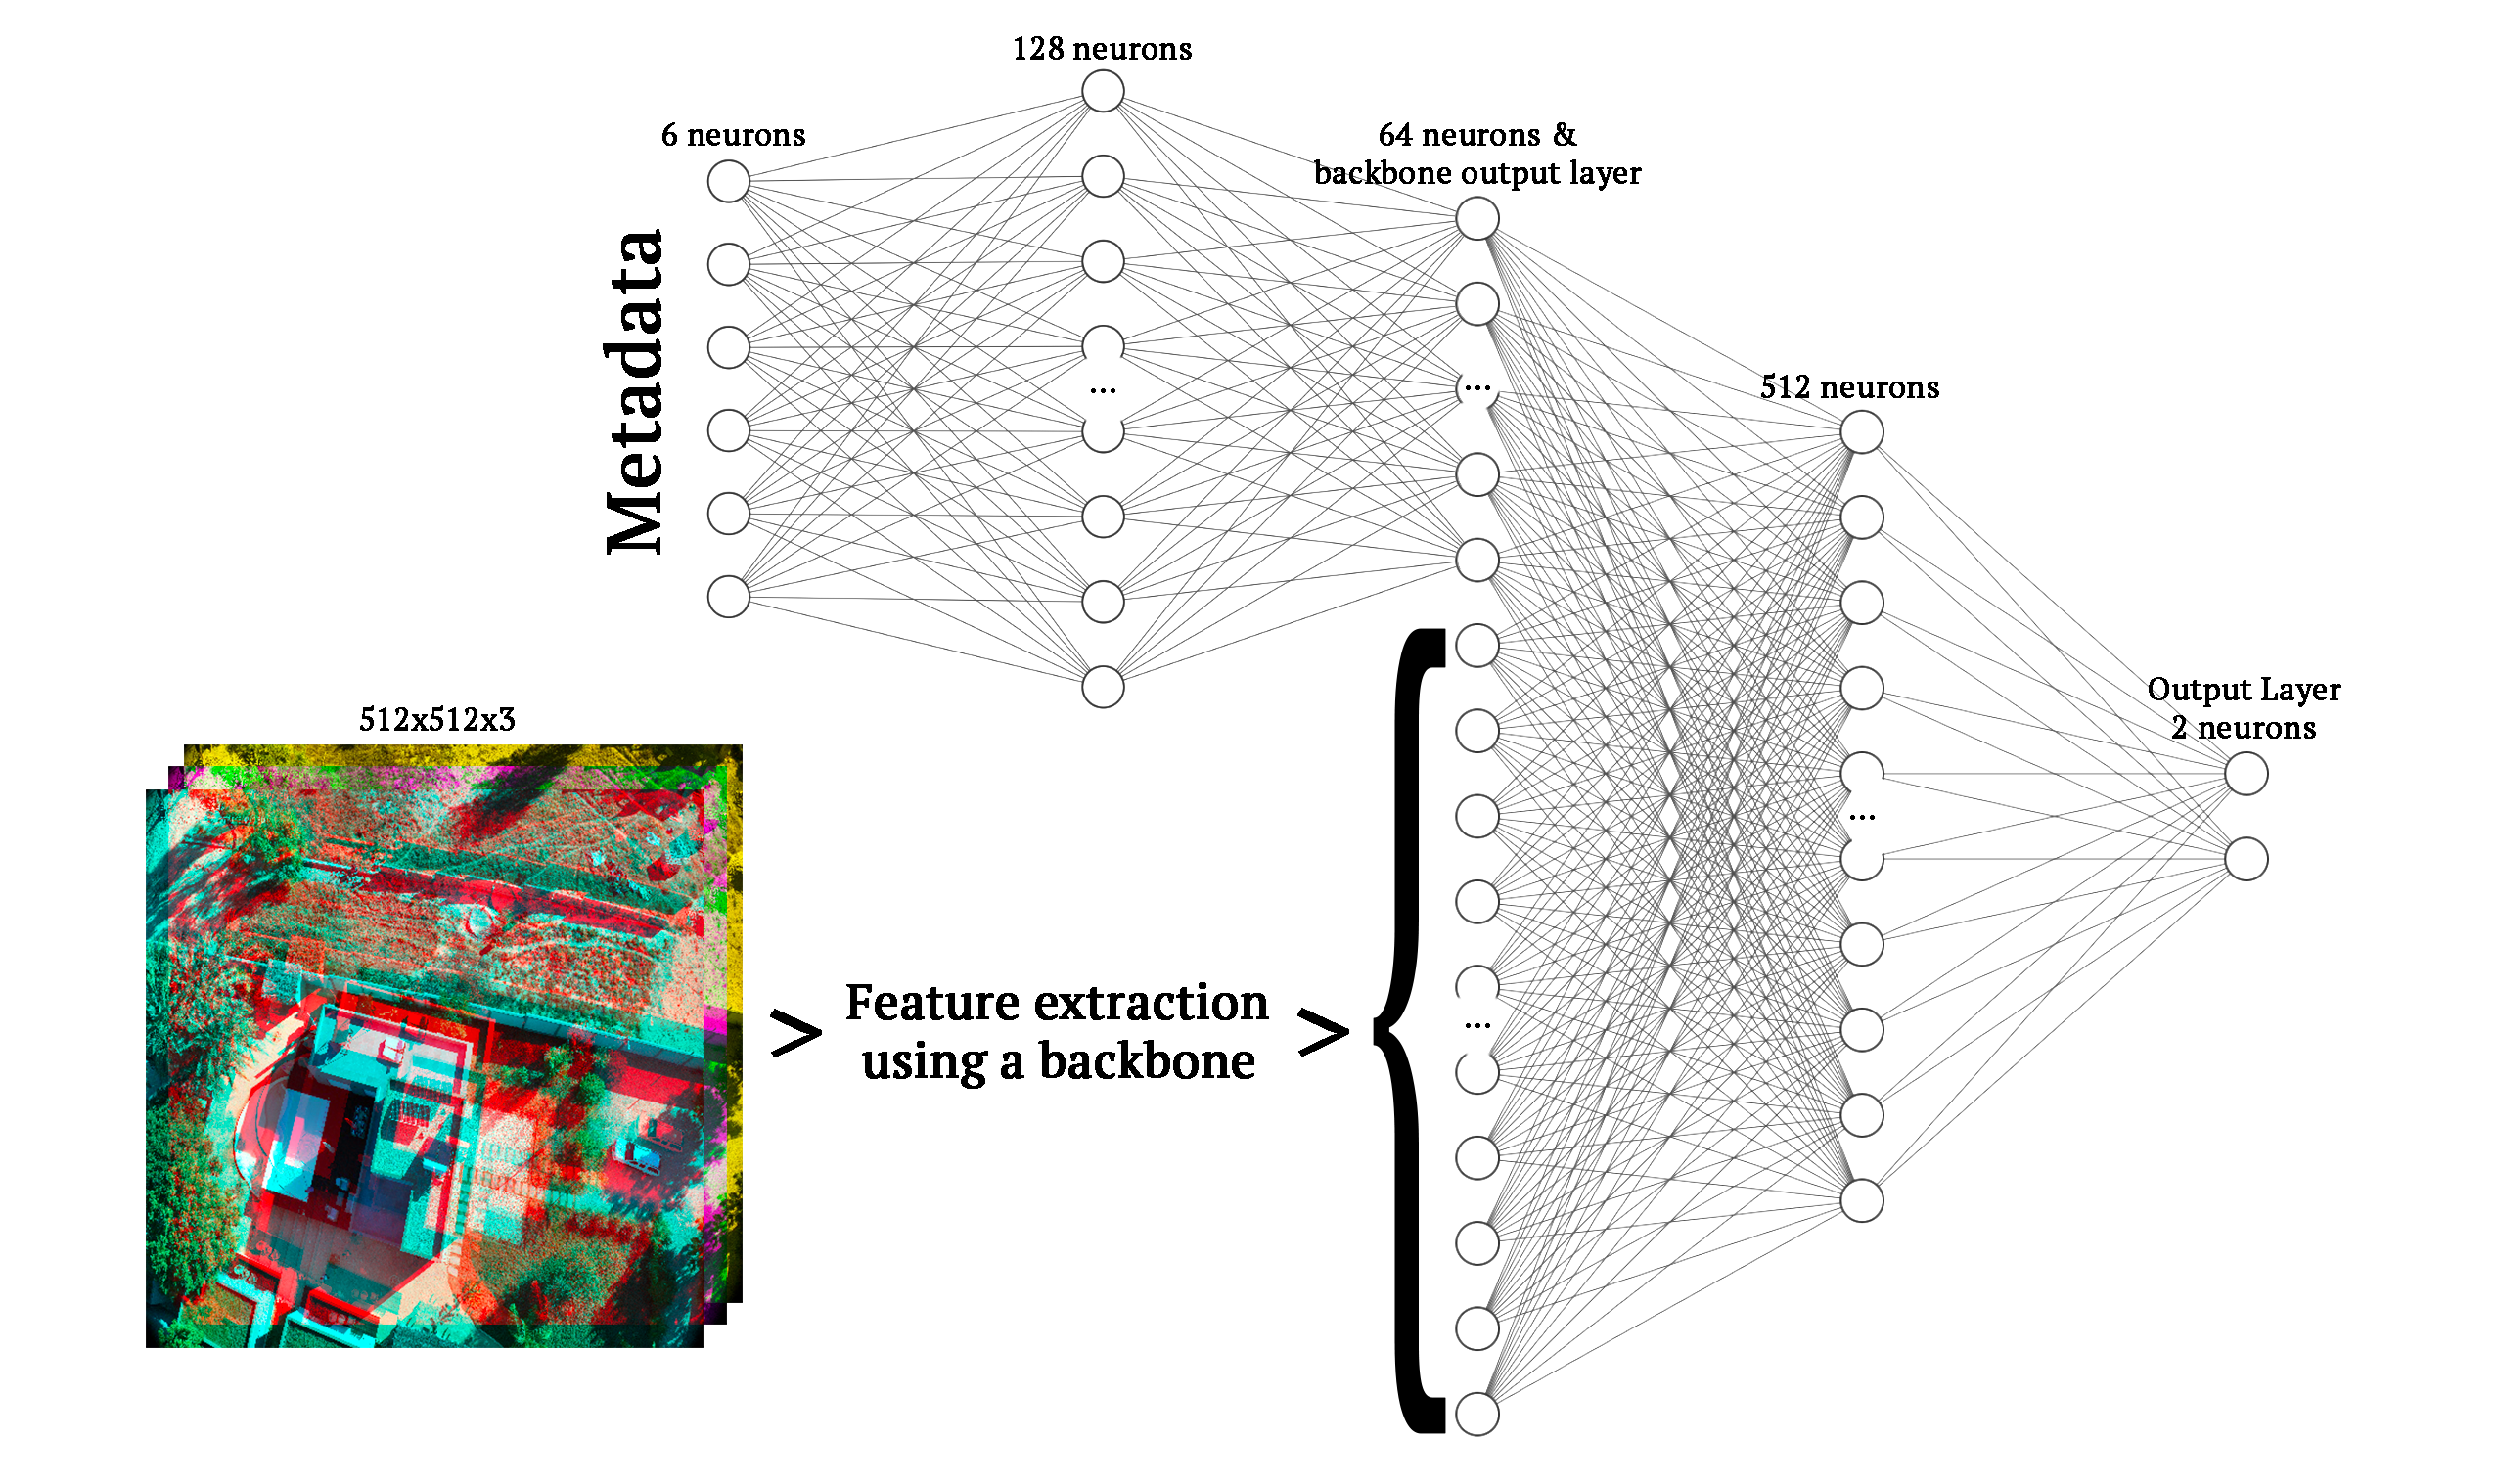
\includegraphics[width=1\linewidth]{assets/nn.png}
    \caption{Architecture of the model shared by user zulo40 in the discussion forums. \cite{zulo4thewin}}
    \label{fig:nn}
\end{figure}

After feature extraction, the data is processed through fully connected layers, followed by a multi-head attention mechanism to enhance the embeddings. The multi-head attention mechanism is an important technique of CNN from the Transformers architecture, whereby the \textit{attention} (i.e., the importance of certain features) is estimated several times in parallel, allowing the model to learn different patterns and relationships between different sets of features. Finally a regression head predicts the number of panels (photovoltaic and thermal solar) in a given image.

The backbones tested were DenseNet121, EfficientNetv2B3 and ResNet101, and after an initial assessment, EfficientNetv2B3 achieved the best performance and the hyperparameters were further fine-tuned with the ranges specified in Table \ref{parametroszulp}.

The criterion for the selection of the best model was the MAE (mean absolute error, the metric used in the Zindi challenge), which gave the following hyperparameters marked in bold in Table \ref{parametroszulp}. The hyperparameters were selected for a small number of combinations, given how time consuming training each model is.

\begin{table}[b]
\centering
\caption{Hyperparameter space for the models based of the hybrid model \textit{zulo40}. The bold values correspond to the selected hyperparameters.}
\label{parametroszulp}
\begin{tabular}{ll}
\toprule
\textbf{Hyperparameter} & \textbf{Possible Values} \\
\midrule
Batch size & $\{\mathbf{16}, 32, 64\}$ \\
Optimizer & \textbf{AdamW} \\
Learning rate & $[\mathbf{10^{-5}}, 10^{-3}]$ \\
Weight decay & $[\mathbf{10^{-5}}, 10^{-3}]$ \\
Dropout & $\{0.2, 0.3, \mathbf{0.4}\}$ \\
Scheduler & \textbf{CosineAnnealingWarmRestarts} \\
T\_0 & $\{3, \mathbf{5}, 7, 10\}$ \\
T\_mult & $\{1, \mathbf{2}, 3, 5\}$ \\
Loss & \textbf{HuberLoss} \\
$\delta$ & \textbf{1} \\
\bottomrule
\end{tabular}
\end{table}
\newpage

Upon selecting the best model, the final inference on the test data was done resorting to TTA, Test-Time Augmentation, where the model makes multiple predictions on augmented versions of the same image (e.g., flipping, scaling, cropping). With this, the final result is an average of the group of predictions. The scheduler selected (CosineAnnealingWarmRestarts) dynamically changes the learning rate following a cosine schedule, with a defined period (T\_0 = 5), where at each period the learning rate decays to a minimum, restarting at the highest set learning rate. This allows to prevent convergence to local minima, by passing through higher learning rates periodically, allowing for fine tuning with lower learning rates for longer periods (given T\_mult = 2, where the period increases two fold at each restart).

% JP: Actualizado

The erratic behaviour of the CV loss curve is evident from Fig. \ref{fig:model01_lc}, likely due to the small validation set (20\% of an already small dataset), which leads to variance spikes due to the changing samples within. The training loss is rather smooth, with periodical increases well in line with the scheduler's algorithm (5, 5 + 10, 15 + 20, ...).

\begin{figure}[H]
    \centering
    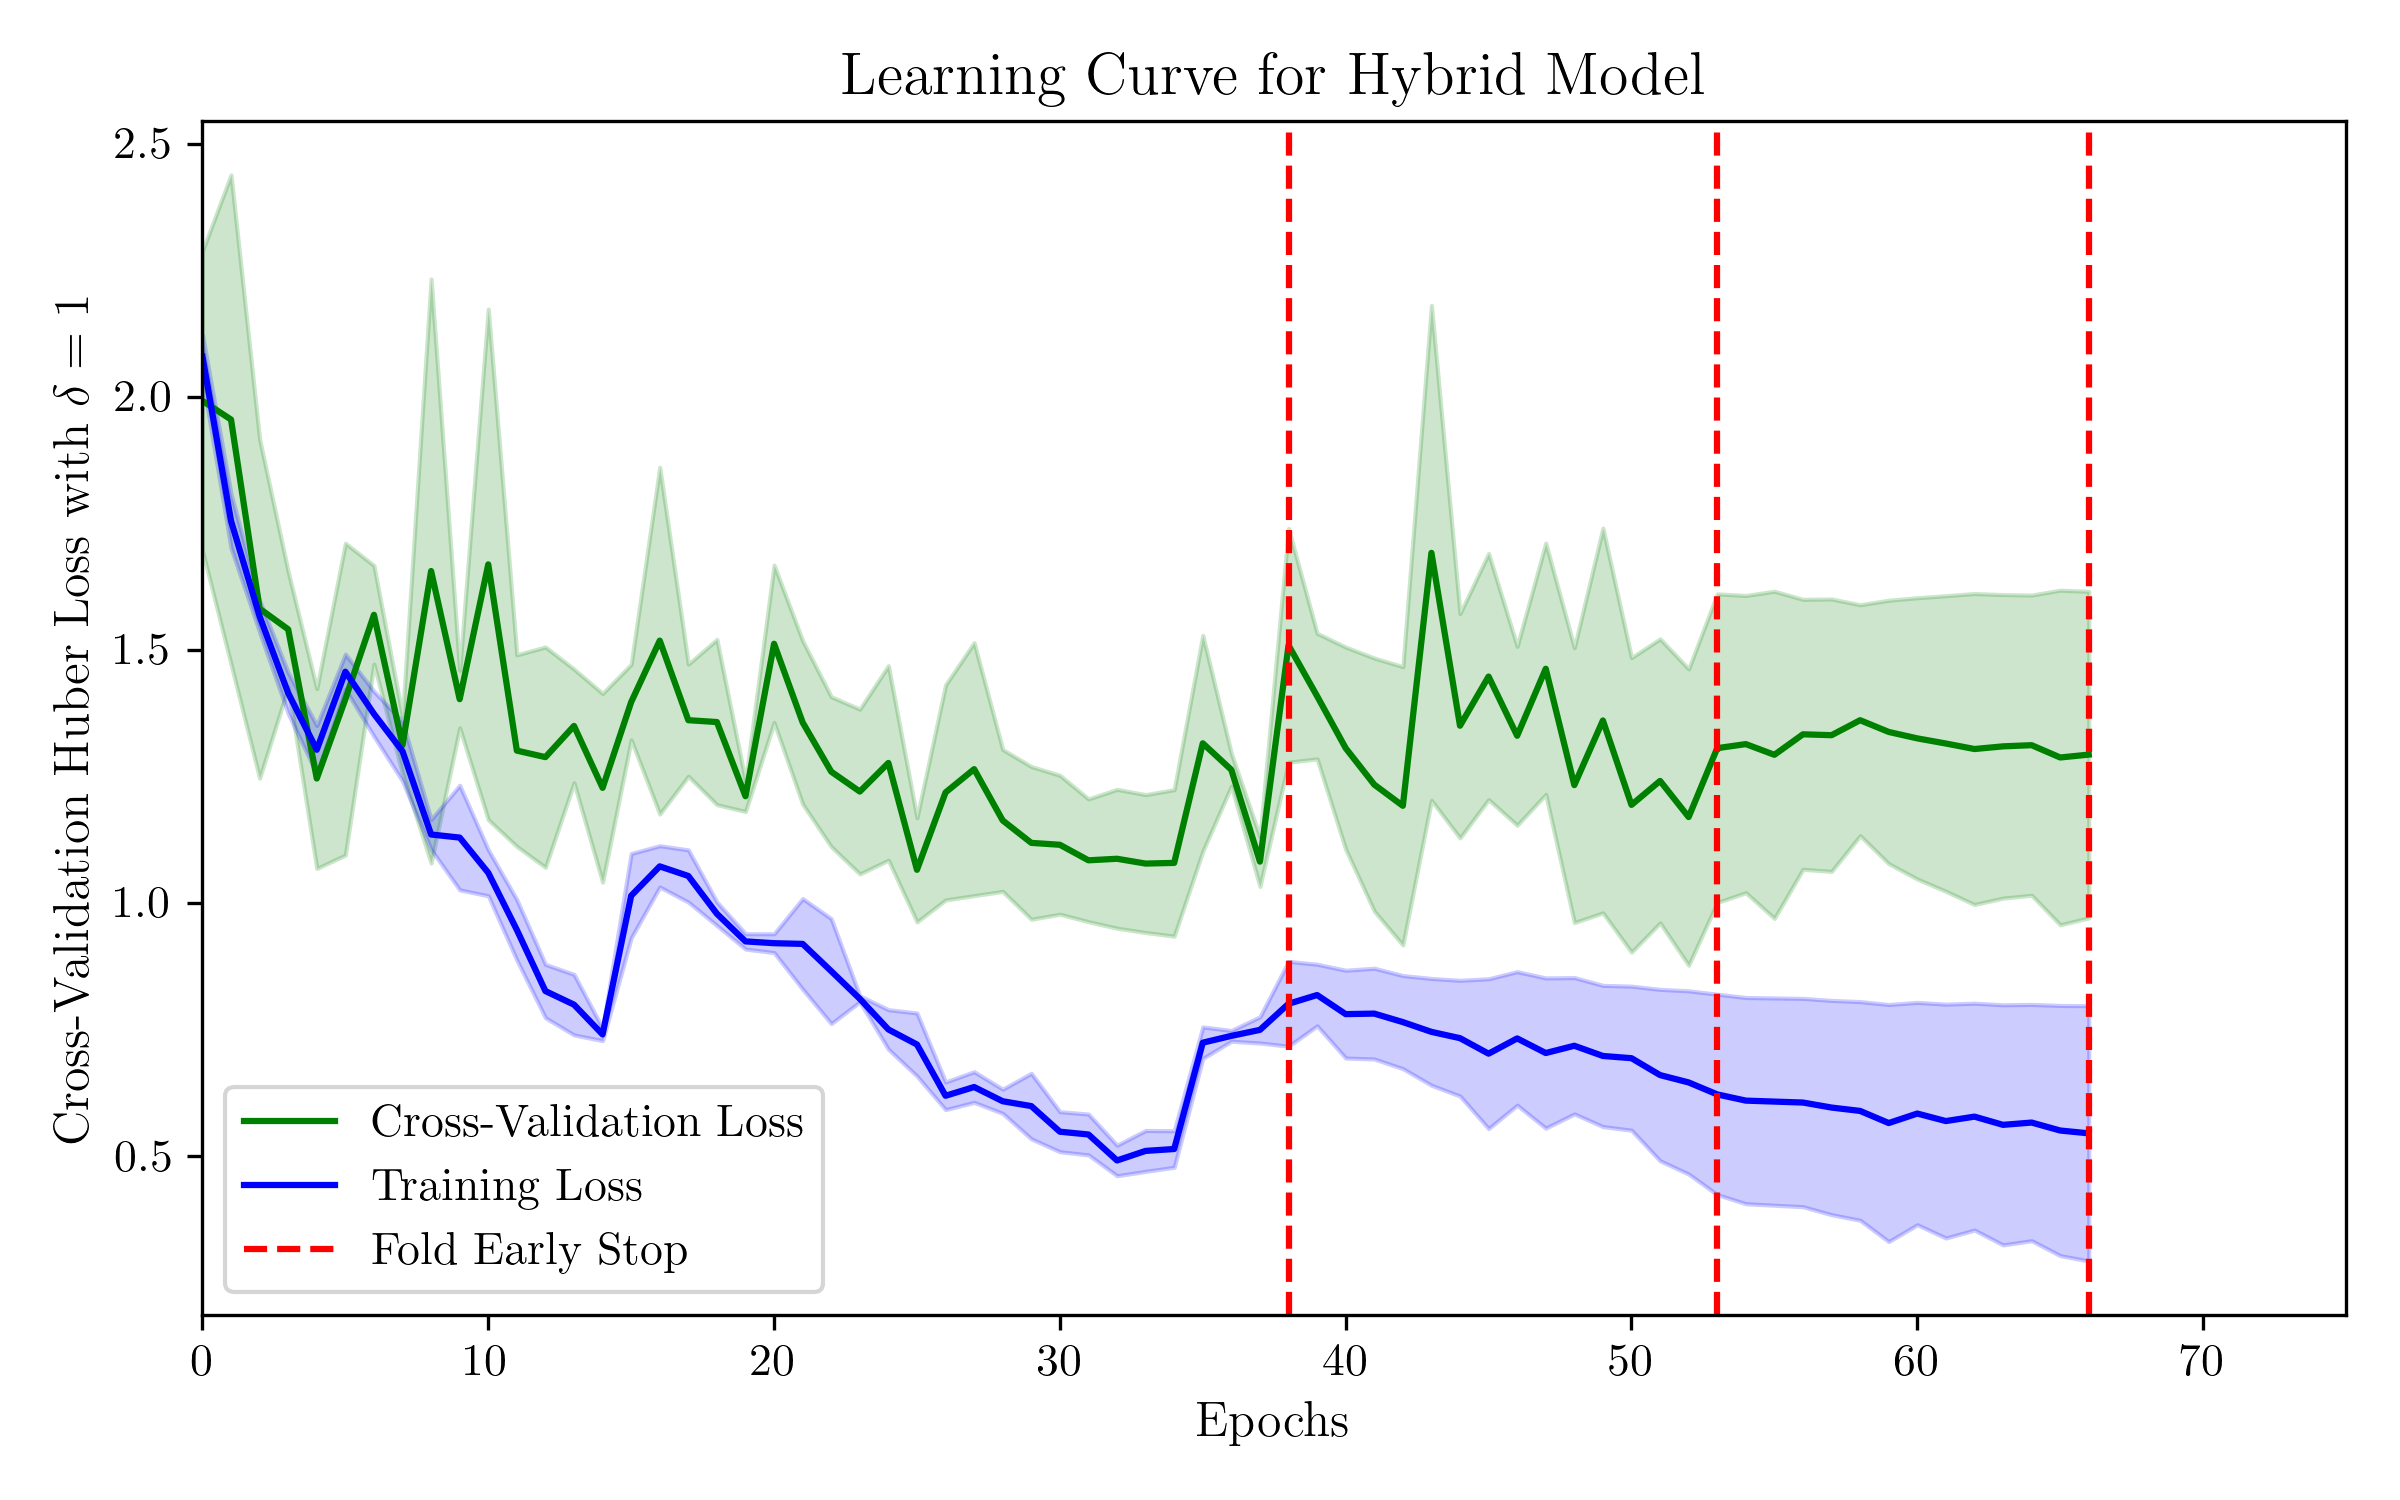
\includegraphics[width=1\linewidth]{assets/model01_lc.png}
    \caption{Learning curve for the best fit model, with Training and Cross-Validation Loss plotted (with standard deviation in shade). The dashed lines correspond to the early stops of each fold.}
    \label{fig:model01_lc}
\end{figure}

The training proceeded for 75 epochs, where the best model was selected based on the lowest validation MAE. From the learning curve, it does not seem to be overfit, but considering the MAE metric and the test set from the Zindi challenge, the test MAE is slightly higher than the training MAE (Table \ref{tab:model01_results}, indicating that the model is not capable of generalizing so well. Despite the slight generalization gap, the overfitting chance can be debatable, as we are dealing with an absolute value metric, which represents a difference of less than half a panel per prediction. 

\begin{table}[H]
\centering
\caption{Error metrics for the Hybrid Model, for the train and test set, along with the number of samples for each.}
\label{tab:model01_results}
\begin{tabular}{lccc}
\toprule
\textbf{Dataset} & \textbf{MAE} & \textbf{Support} \\
\midrule
Train Set & 0.5127 & 3312 \\
Test Set & 0.8434 & 1107 \\
\bottomrule
\end{tabular}
\end{table}

\subsection{Object Detection}

Upon initial testing of YOLO models in the dataset, it was clear from the beginning that the labelling style posed a major hindrance to the type of models relying on masks/labels, which resulted in significant loss in performance. Based on this assessment, an individual review of roughly 200 images was conducted and individual masks for each panel (either solar thermal or photovoltaic) were created, which resulted in roughly 1000 individual masks (mostly for photovoltaic). To train these models, only images with individual masks were considered, resulting in a reduction in size of the dataset of roughly 40\%. The remaining individual masks were transformed to bounding box notation (COCO notation style).

As for the previous section, the criterion for selecting the best model was the MAE. A small number of hyperparameter combinations was tested, due to the time-consuming nature of training. The possible values considered for each hyperparameter are listed in Table \ref{parametrosobjid}.

% ORGANIZAR TABELA
\begin{table}[H]
\centering
\caption{Hyperparameter space for the YOLO model. The bold values correspond to the selected hyperparameters. The remaining parameters are left as default.}
\label{parametrosobjid}
\begin{tabular}{ll}
\toprule
\textbf{Hyperparameter} & \textbf{Possible Values} \\
\midrule
Batch size & $\{16, \mathbf{32}\}$ \\
Model & \{\textbf{yolov8l}, yolo11m, yolo11l\} \\
Image size & \textbf{512} \\
Augmentation & \textbf{True} \\
Early stopping patience & $[15, \mathbf{25}]$ \\
cls & $[0.5, \mathbf{1.5}]$ \\
lr0 & $[\mathbf{10^{-5}}, 10^{-3}]$ \\
lrf & $[0.1, \mathbf{1}]$ \\
mixup & $[0, \mathbf{0.75}]$ \\
copy\_paste & $[0, \mathbf{0.75}]$ \\
scale & $[0.5, \mathbf{1}]$ \\
\bottomrule
\end{tabular}
\end{table}

From the different model fits, Fig. \ref{fig:model03_mae_boxplot} displays the MAE ranges using boxplots. The YOLOv8L model, for instance, was trained three times with distinct hyperparameter sets, highlighting the importance of tuning. The model with the lowest mean MAE was selected (YOLOv8L-3), and its corresponding hyperparameters are marked in bold in Table \ref{parametrosobjid}.

\begin{figure}[H]
    \centering
    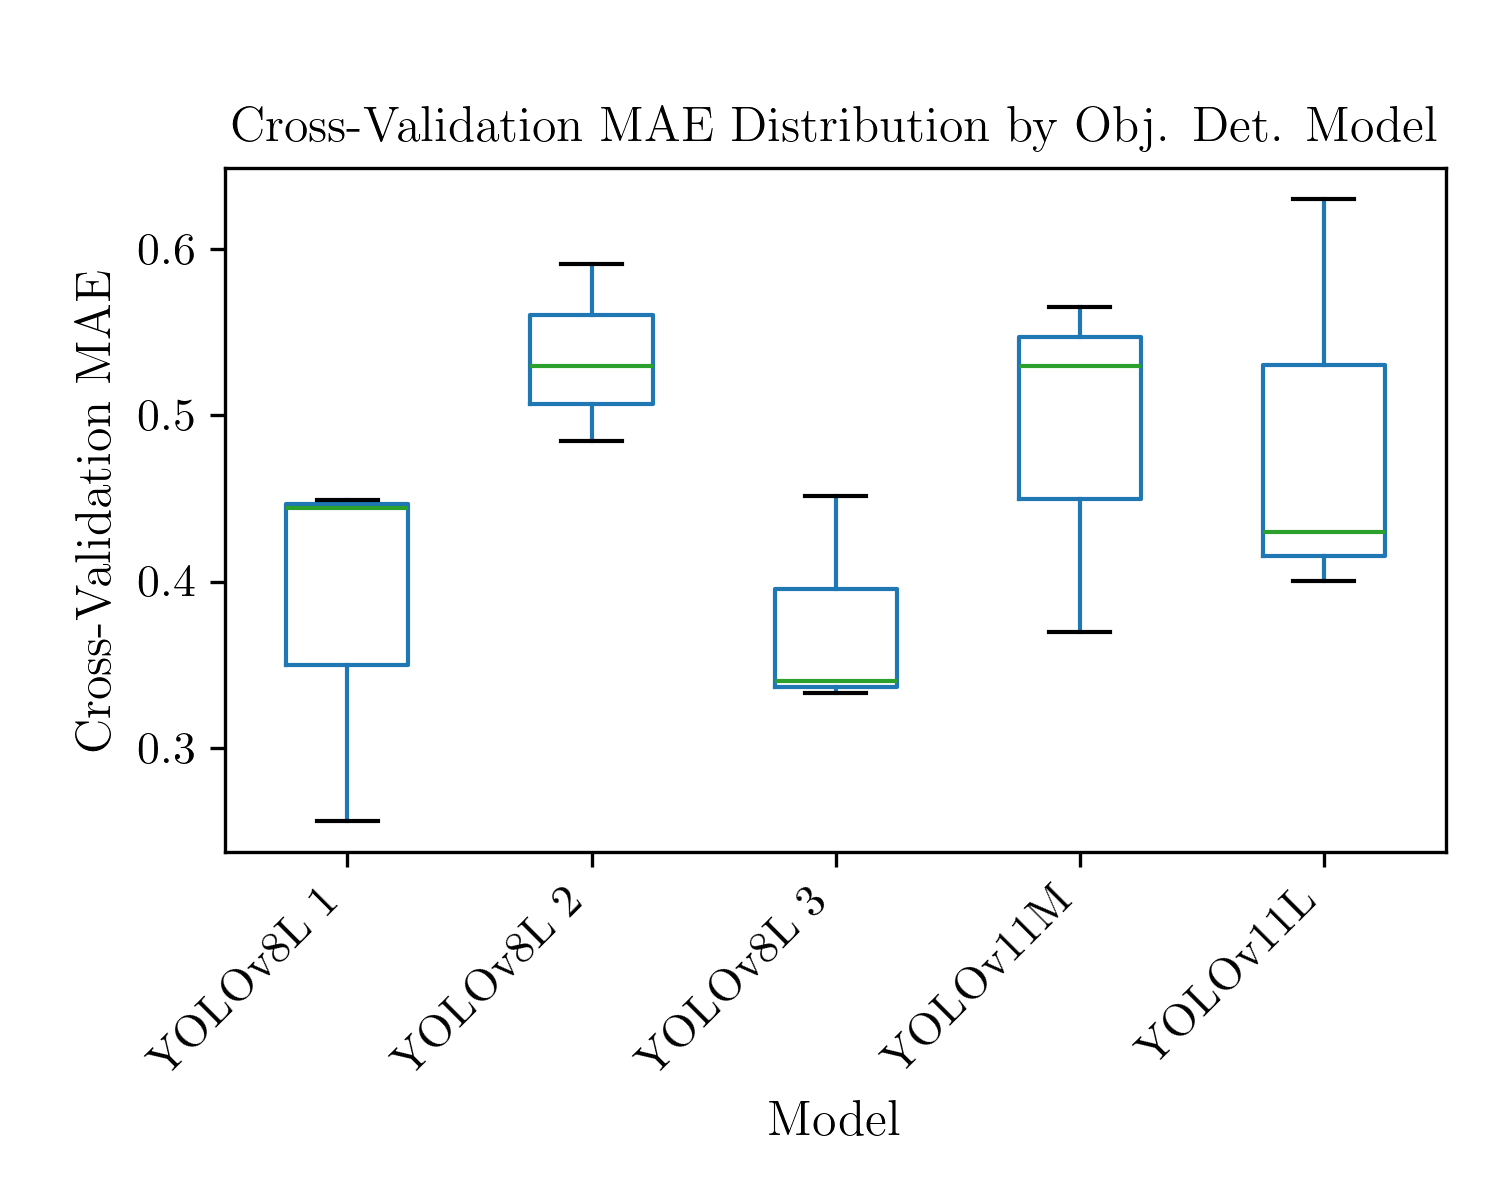
\includegraphics[width=1\linewidth]{assets/model03_mae_boxplot.png}
    \caption{CV MAE for each model. Each boxplot represents the values obtained during the cross validation of each model.}
    \label{fig:model03_mae_boxplot}
\end{figure}

The results from the best model are shared below, although one should bear in mind that the metrics shared are for the model's main goal (i.e., object identification), and only after the training it was possible apply the model to the test set and count the number of panels of each kind.

Unlike in the previous section, the cross-validation and training loss curves (Fig. \ref{fig:model03_lc}) do not evidence the spikes seen before (no learning rate scheduler used), but the axis scale might deceive the interpretation: the cross-validation loss still has a considerable variance in comparison with the training loss curve. This still is due to the difficulty in generalizing the learning, with such small dataset. Despite this fact, the learning curves progress well and do not evidence overfitting, although the variance of the training curve increases drastically at the very late stages of training. One aspect to notice is how the CV loss curve is below the training loss: which might seem strange, but due to the heavy augmentation and the usage of parameters that target class imbalance (copy\_paste = 0.75; mixup = 0.75) the model has a harder time learning the features of the target objects.

The resulting F1-Confidence curve (Fig. \ref{fig:model03_yolof1}) is a typical analysis for this type of models, as it relates two important metrics: F1-score, which is a result of the precision and recall of the predicted samples; and confidence, which consists of the product of the probability of a given object existing within the bounding box, and the probability of a given class given that object is in the box. The equation for confidence is available below.

\[
\text{Confidence} = P(\text{object}) \times P(\text{class} \mid \text{object})
\]

\begin{figure}[H]
    \centering
    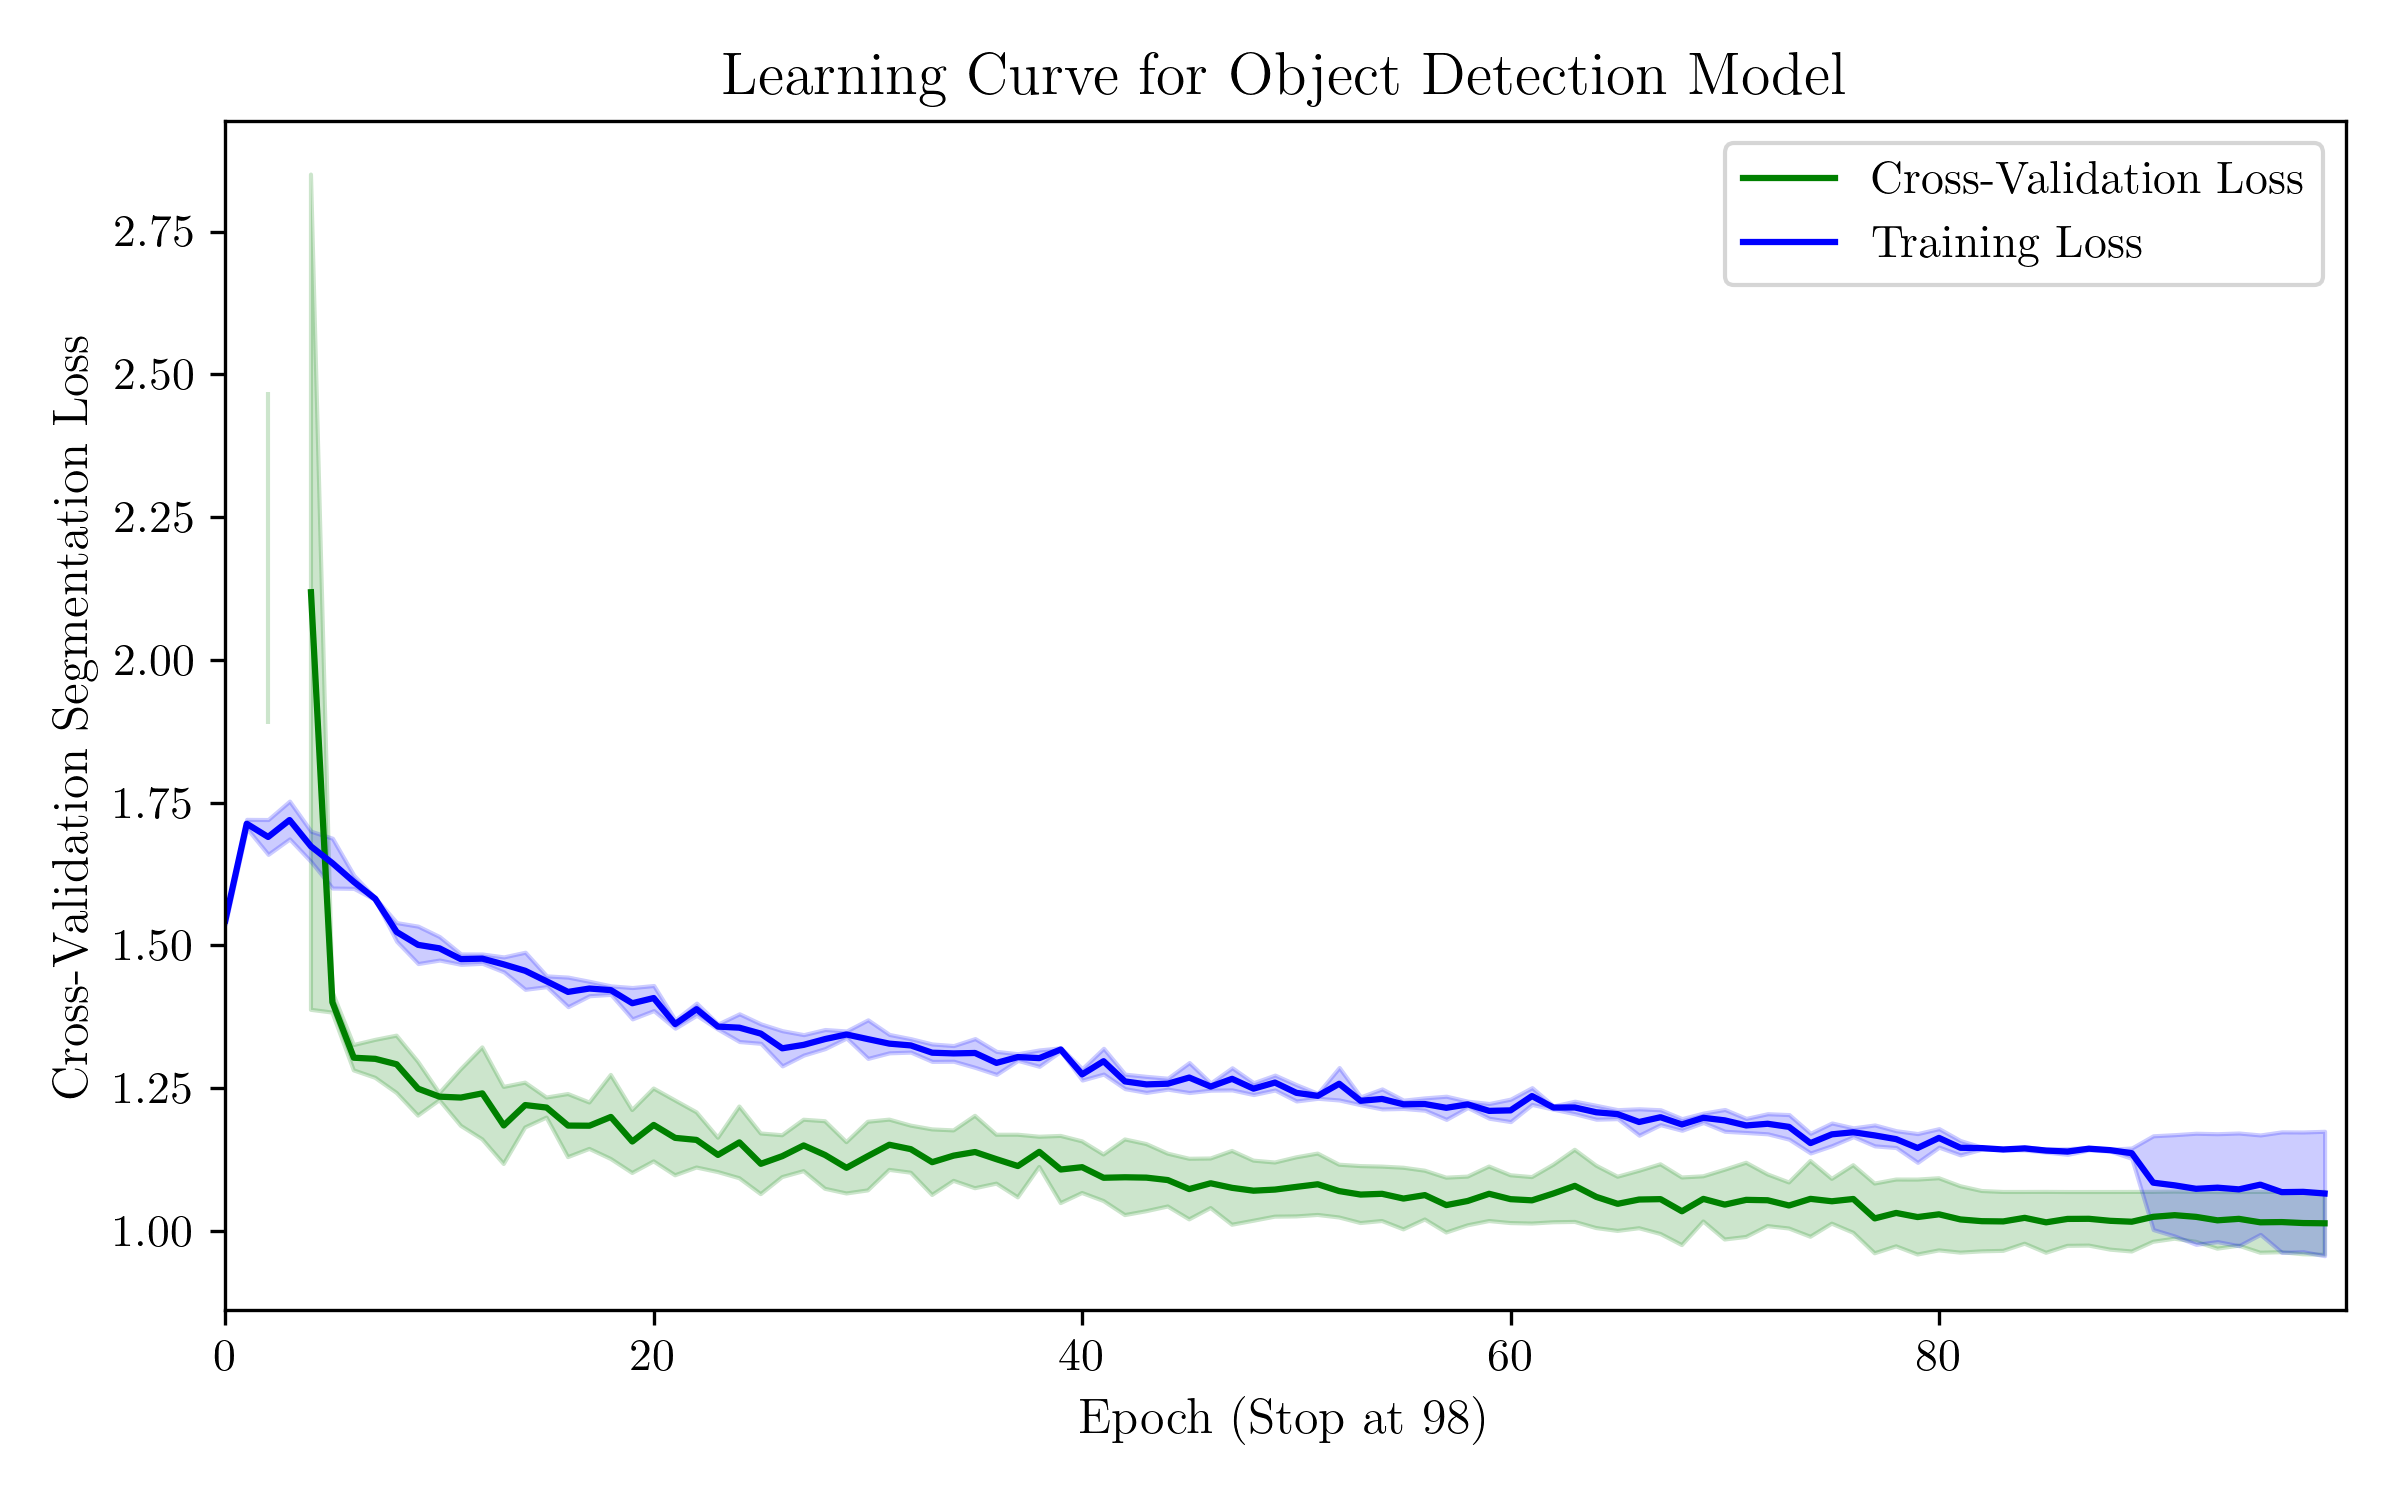
\includegraphics[width=1\linewidth]{assets/model03_lc.png}
    \caption{Learning curve for YOLOv8L-3, with
Training and Cross-Validation Loss plotted (with standard
deviation in shade). The dashed lines correspond to the early stops of each fold.}
    \label{fig:model03_lc}
\end{figure}

%\textbf{não nos podemos esquecer de referenciar o código usado)}




Moreover, confidence is a result of the training process, where during each image passes through the CNN the probabilities for objectness (i.e., presence of object) and class are learned from training. This output serves as the final layer's activation, shaped by the training, which will reflect the training and be used during inference stage to assess detection certainty.

The evaluation of predictions (i.e., evaluating true/false positive/negative) is based on IoU (Intersection over Union), comparing the predicted mask ($B_{\text{p}}$) with the ground-truth ($B_{\text{gt}}$) for that image. It also allows to avoid the usage of overlapping predictions, removing redundant bounding boxes.

\[
\text{IoU} = \frac{\text{Area of } (B_p \cap B_{gt})}{\text{Area of } (B_p \cup B_{gt})}
\]

The highest F1-score in the range is 0.80 from early confidence of 0.35, with both classes following closely at the top of the F1-score range for most of the confidence interval.

\begin{figure}[H]
    \centering
    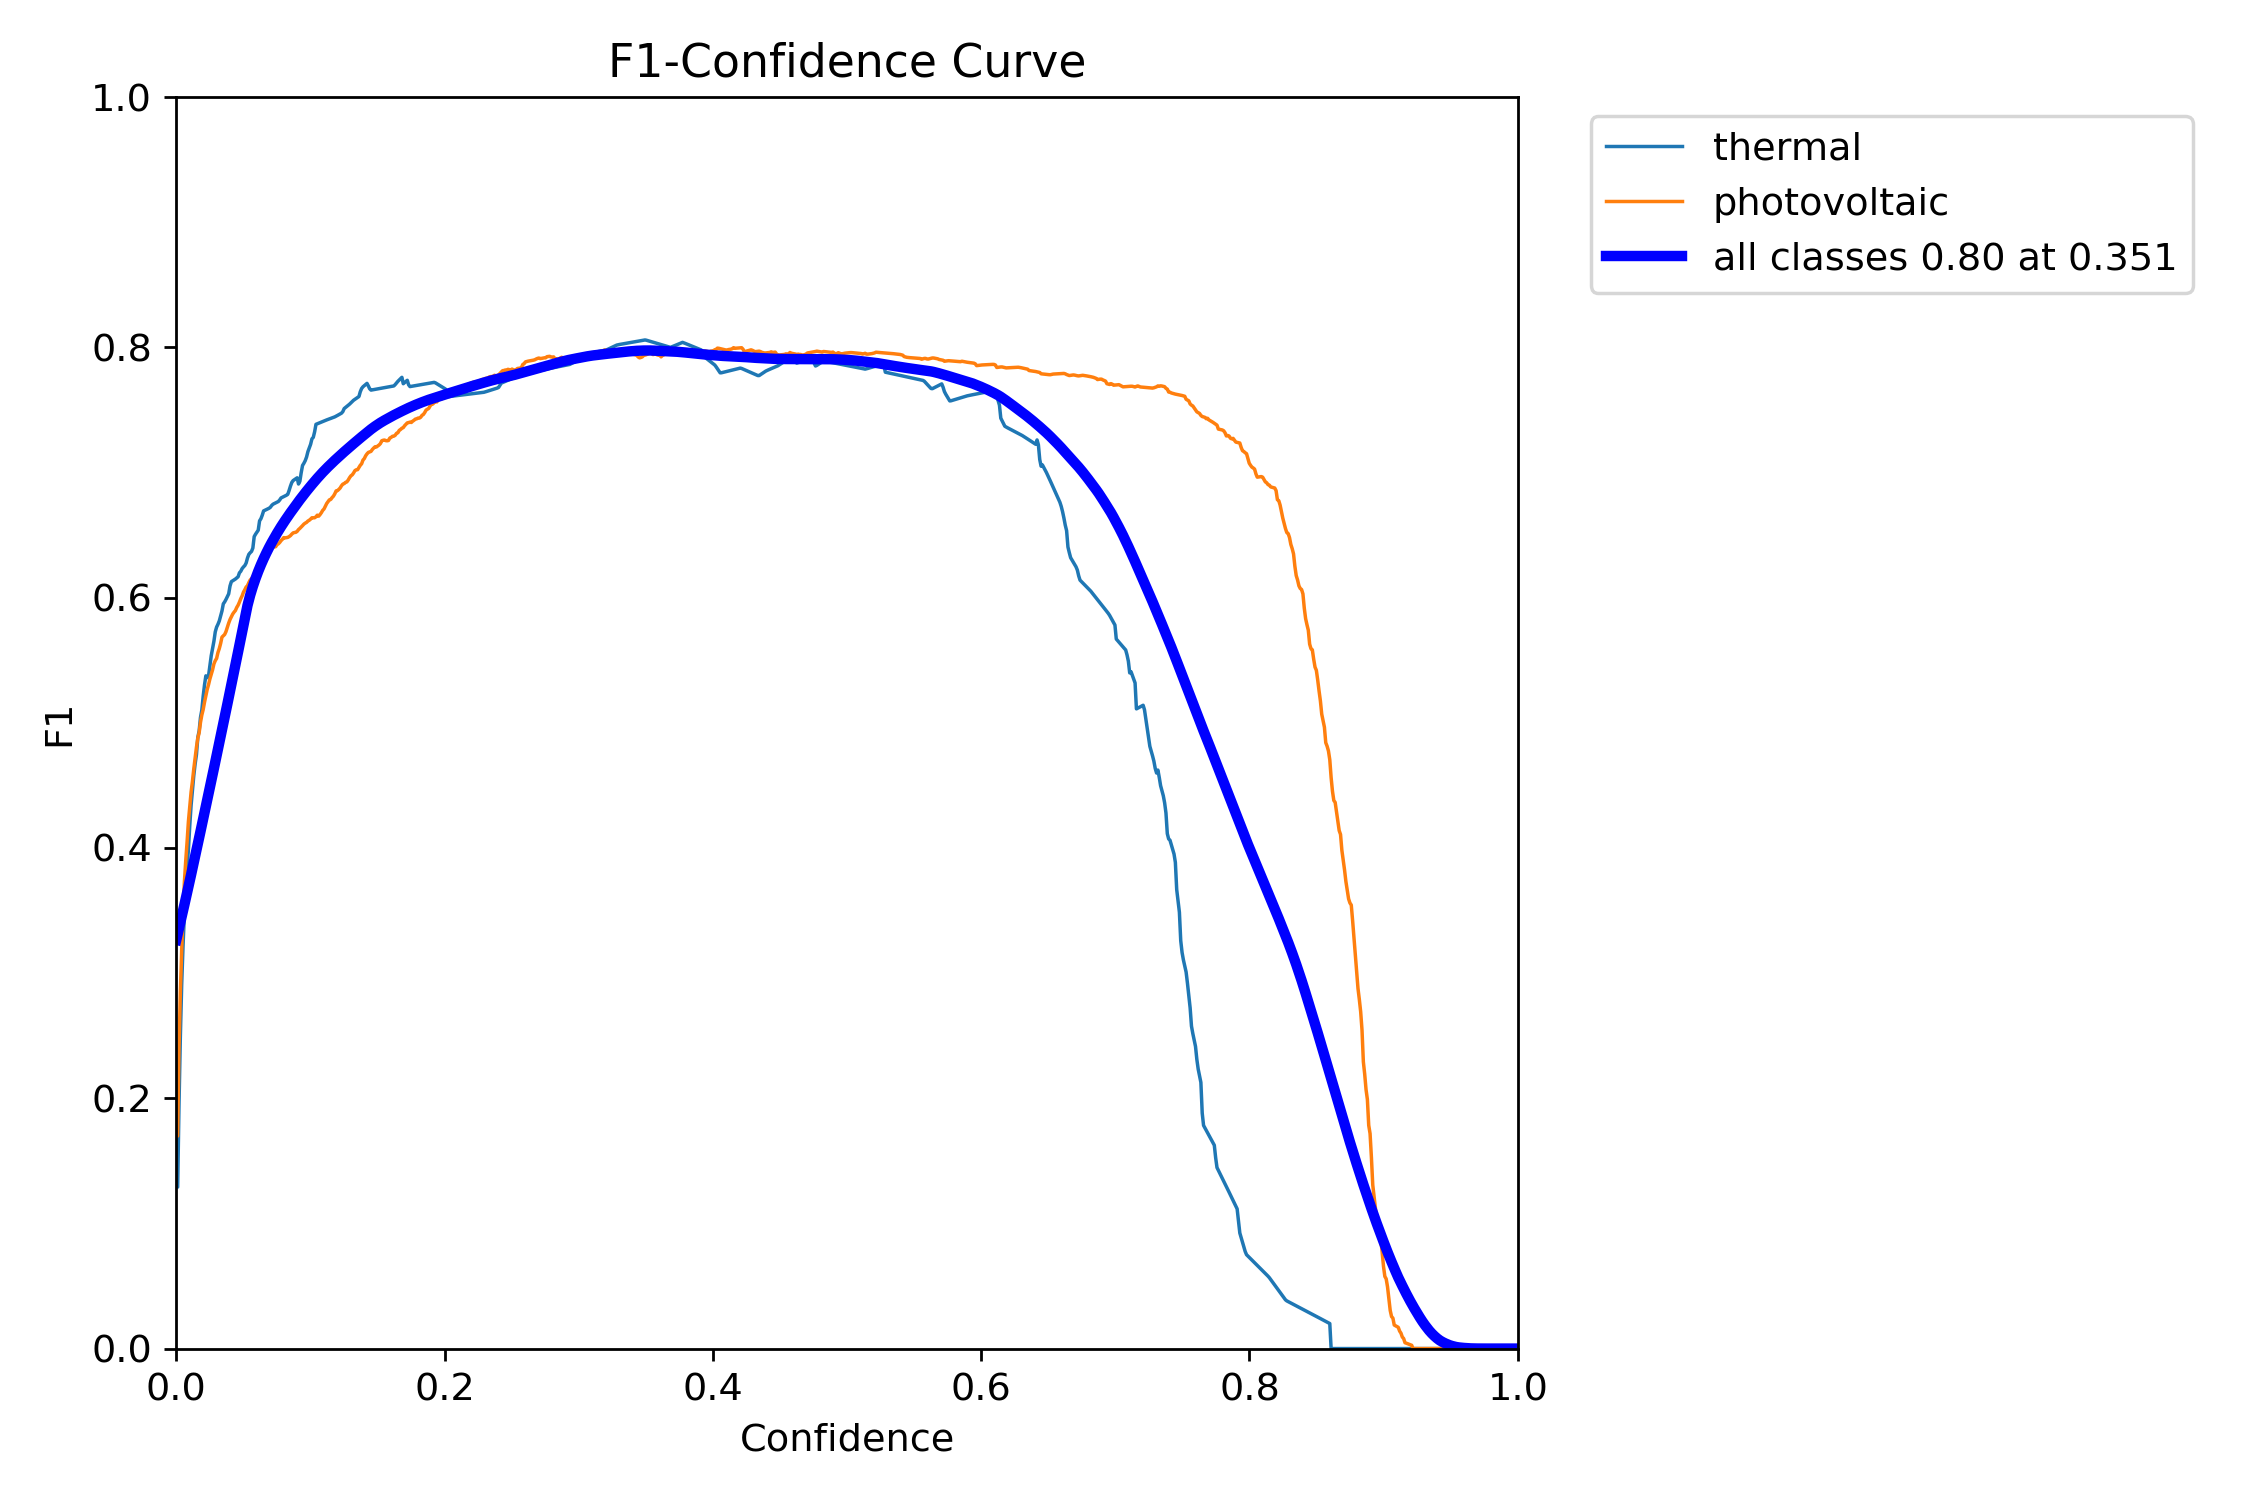
\includegraphics[width=1\linewidth]{assets/model03_yolof1.png}
    \caption{F1-Confidence curves for YOLOv8L (graph automatically generated from the ultralytics package.}
    \label{fig:model03_yolof1}
\end{figure}

Despite efforts to achieve a better model, the MAE of the train and test sets were among the worst evaluated, especially when considering how low the MAE for CV training was.

\begin{table}[H]
\centering
\caption{Error metrics for the Object Detection Model, for the train and test set, along with the number of samples for each.}
\label{tab:model03_results}
\begin{tabular}{lccc}
\toprule
\textbf{Dataset} & \textbf{MAE} & \textbf{Support} \\
\midrule
Train Set & 1.4330 & 3312 \\
Test Set & 1.2645 & 1107 \\
\bottomrule
\end{tabular}
\end{table}

\subsection{Instance Segmentation}

Using the same labels prepared in section \textit{B.}, the different models were fit for random combinations of hyperparameters, as  listed in Table \ref{parametrosseg}.

%o conjunto de pesquisa de hyperparemetros é dado pela tabela seguinte, mas é de notar q nsao sao testadas todas as combinacoes mas apenas algumas aleatorias


\begin{table}[H]
\centering
\caption{Hyperparameter space for the YOLO-seg model. The
bold values correspond to the selected hyperparameters. The remaining parameters are left as default.}
\label{parametrosseg}
\begin{tabular}{ll}
\toprule
\textbf{Hyperparameter} & \textbf{Possible Values} \\
\midrule
Batch size & $\{\mathbf{8}, 32, 16\}$ \\
Model & \{yolov8l-seg, yolo11m-seg, \textbf{yolo11l-seg}\} \\
Image size & \textbf{512} \\
Augmentation & \textbf{True} \\
Early stopping patience & $[10, \mathbf{25}]$ \\
cls & $[\mathbf{0.5}, 2.5]$ \\
lr0 & $[10^{-4}, \mathbf{10^{-3}}]$ \\
lrf & $\{0.01, \mathbf{0.1}, 1\}$ \\
mixup & $[\mathbf{0}, 0.5]$ \\
copy\_paste & $[\mathbf{0}, 0.8]$ \\
scale & $[\mathbf{0.5}, 1]$ \\
\bottomrule
\end{tabular}
\end{table}

The MAE of the different folds for the models listed are presented in Fig. \ref{fig:model02_mae_boxplot} are represented as boxplots, where the best model (YOLOv11L-1) was selected for further analysis.

\begin{figure}[H]
    \centering
    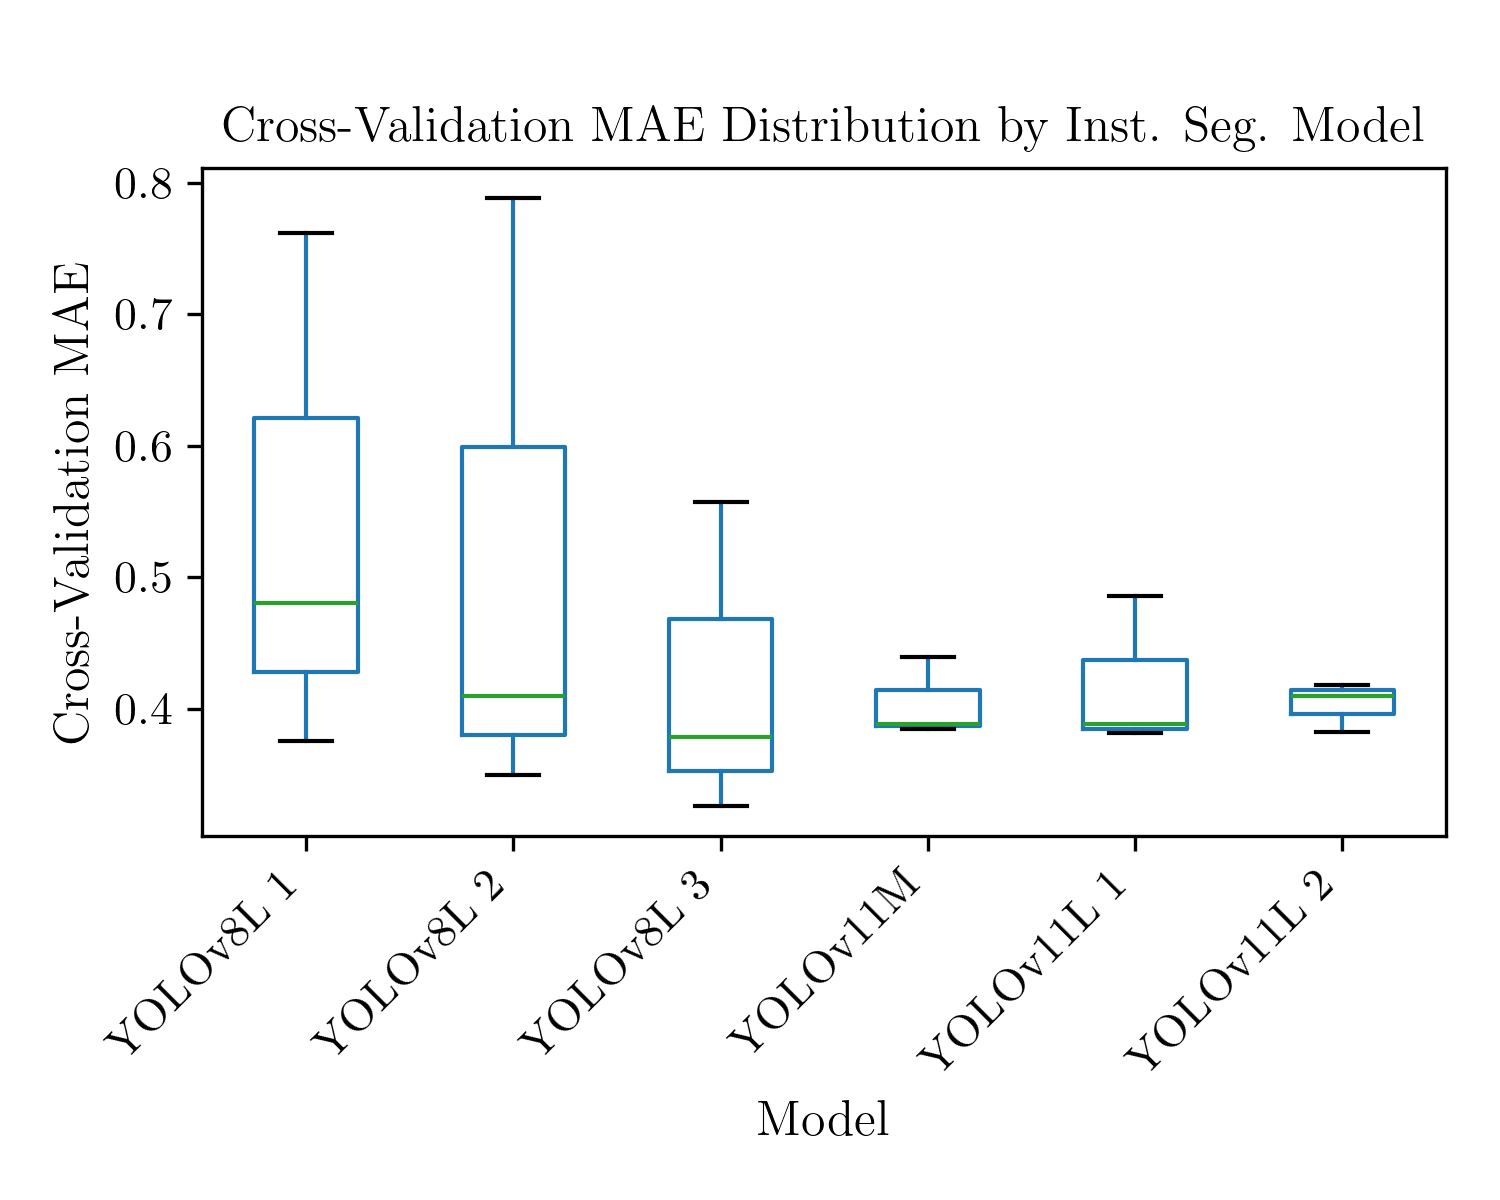
\includegraphics[width=1\linewidth]{assets/model02_mae_boxplot.png}
    \caption{CV MAE for each model. Each boxplot represents the values obtained during the cross validation of each model.}
    \label{fig:model02_mae_boxplot}
\end{figure}

In Fig. \ref{fig:model02_lc} the CV loss curve stabilizes early on, whereas the training loss decreases until around the 80\textsuperscript{th} epoch, after which, one of the folds keeps training but not diminishing the loss significantly. The fact that the CV loss does not change throughout the training is telling of how the model struggled to learn and generalize the features from the dataset. This might well be due to the reduced dataset size (mentioned previously), and the fact that some of the ideal hyperparameters (copy\_paste = 0; mixup = 0) did not promote replication of the minority class. The training of the longest fold stopped at the 92\textsuperscript{nd} epoch due to early stopping.

\begin{figure}[H]
    \centering
    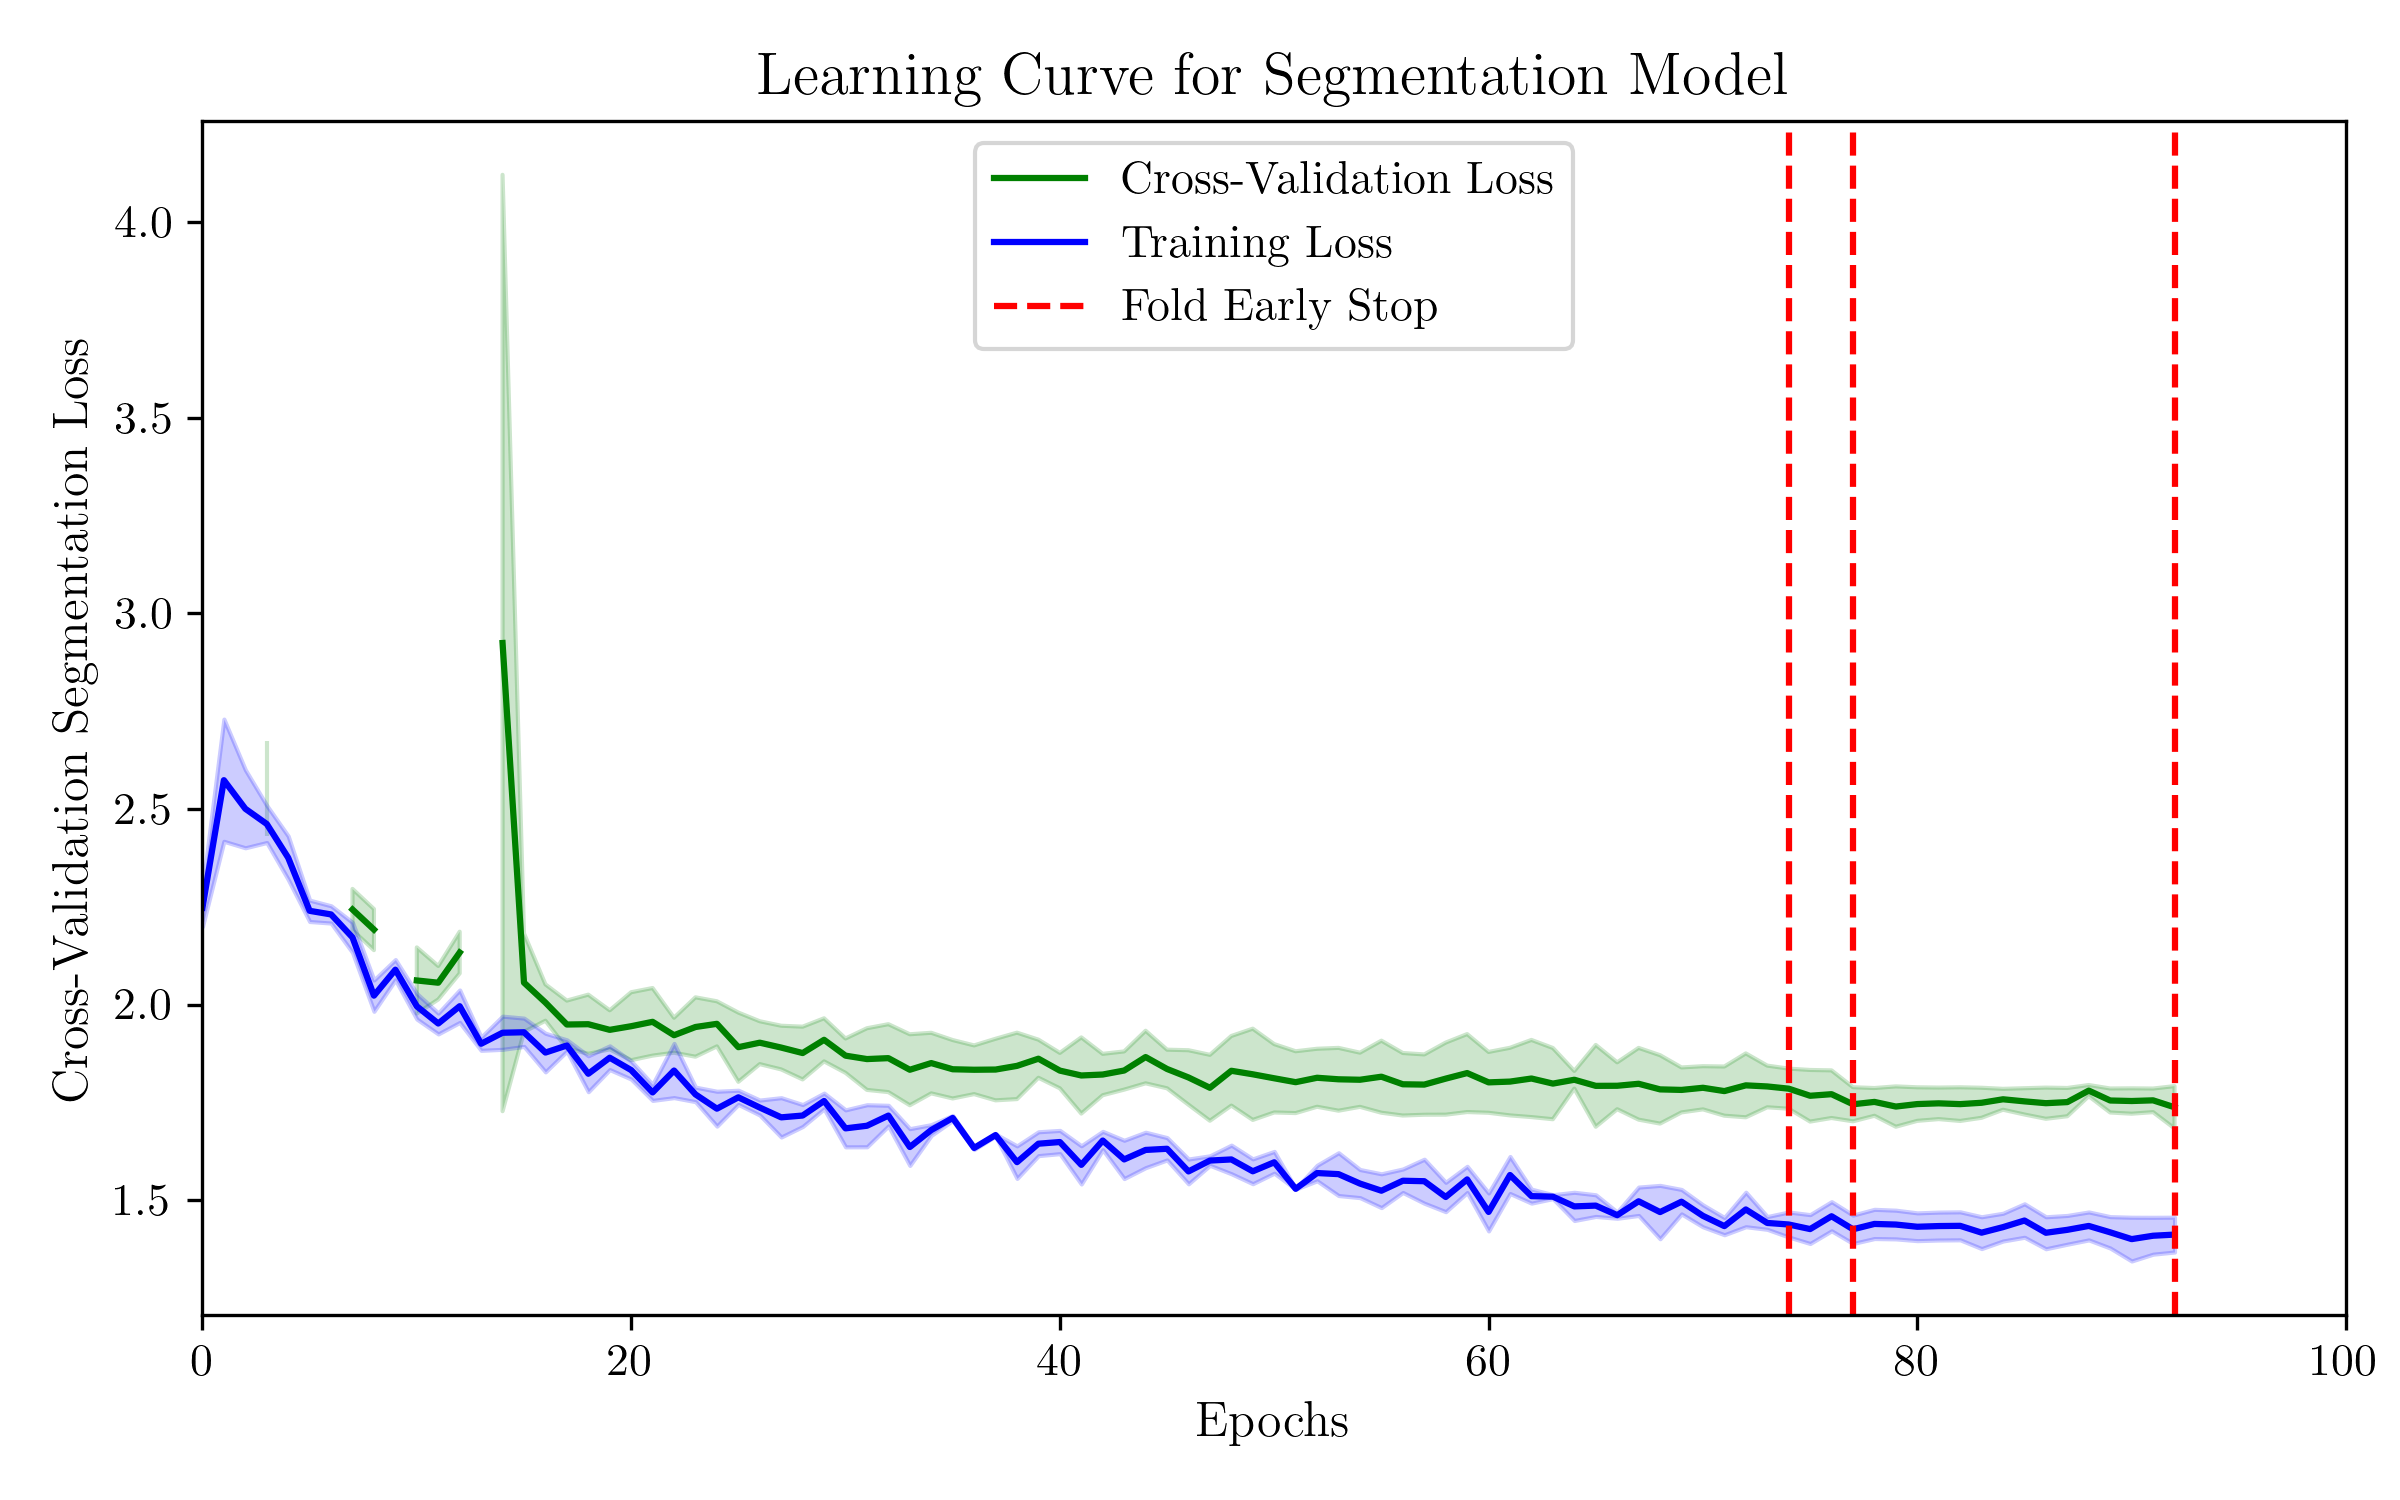
\includegraphics[width=1\linewidth]{assets/model02_lc.png}
    \caption{Learning curve for YOLOv11L-2, with Training and Cross-Validation Loss plotted (with standard deviation in
shade). The dashed lines correspond to the early stops of each fold.}
    \label{fig:model02_lc}
\end{figure}

For the F1-Confidence curve (Fig. \ref{fig:model02_yolof1}) all classes attain F1-score of 0.76 at 0.46, which is a lower F1-score and narrower confidence range than the object detection model. The class curves also follow very distinct trends, with the F1-score of the thermal solar panels being considerably worse than that of the photovoltaic panels.

\begin{figure}[H]
    \centering
    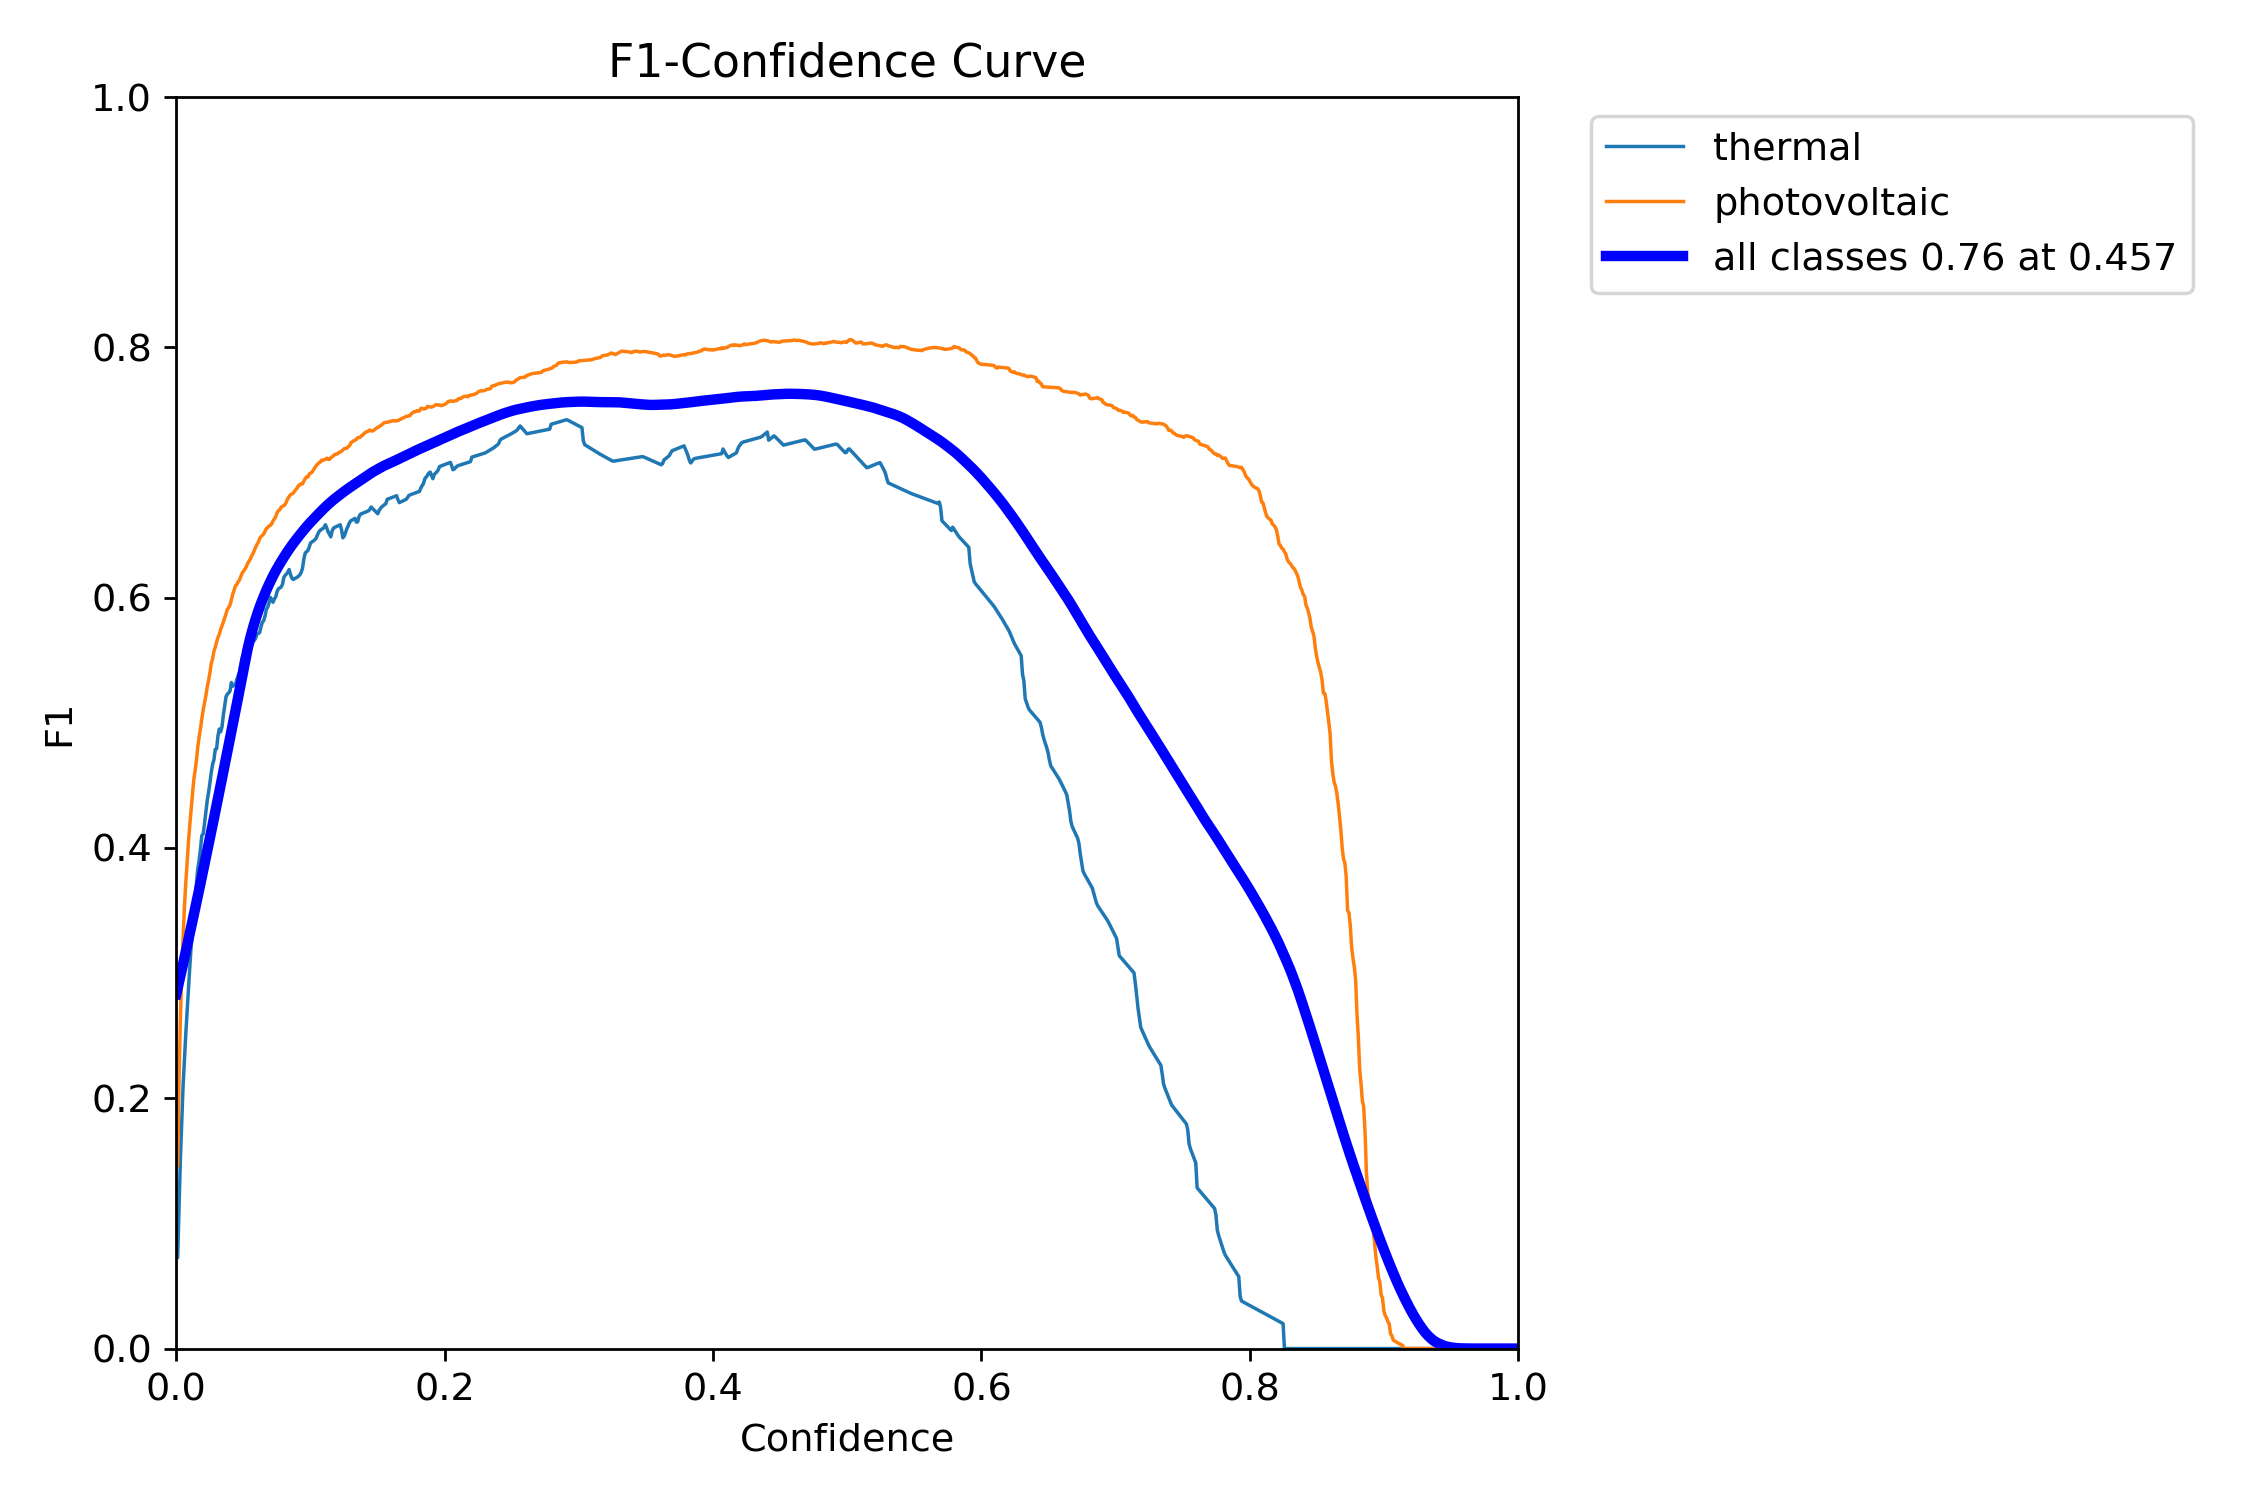
\includegraphics[width=1\linewidth]{assets/model02_yolof1.png}
    \caption{F1-Confidence curves for YOLOv11L-2 (graph automatically generated from the ultralytics package).}
    \label{fig:model02_yolof1}
\end{figure}

The MAE for the train and test set is similar, with the MAE for the test set being slightly lower (Table \ref{tab:model02_results}). This is consistent with the results presented, being this the model that performed the worst among the group.

\begin{table}[H]
\centering
\caption{Error metrics for the Segmentation Model, for the train and test set, along with the number of samples for each.}
\label{tab:model02_results}
\begin{tabular}{lccc}
\toprule
\textbf{Dataset} & \textbf{MAE} & \textbf{Support} \\
\midrule
Train Set & 1.5645 & 3312 \\
Test Set & 1.3415 & 1107 \\
\bottomrule
\end{tabular}
\end{table}


\section{Discussion}

In order to provide a representative comparison of the three models, each fold of the final model was used to pass the test set through it and the MAE score was collected from the Zindi Challenge website. The results are shown in Fig. \ref{fig:results_mae_boxplot}, where the Hybrid model clearly shows a lower value of MAE (both on average and range). Both Object Detection and Instance Segmentation show a narrower range of MAE, but worse than the Hybrid model.
\begin{figure}[H]
    \centering
    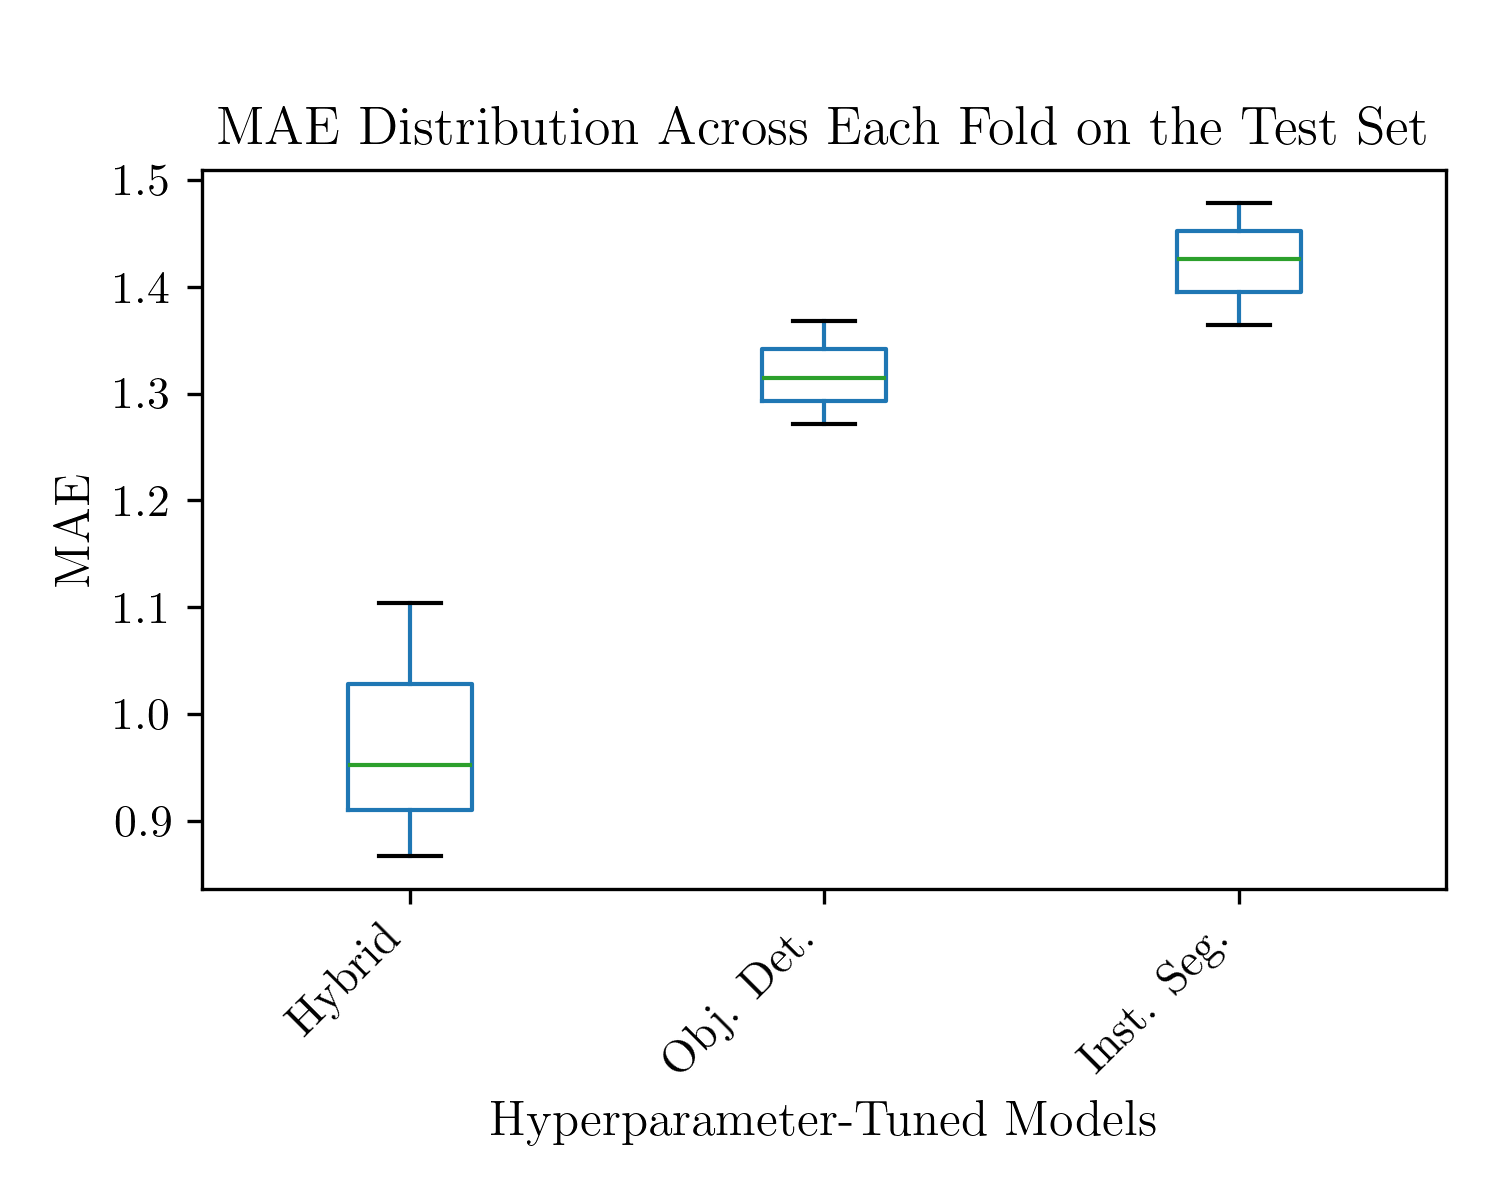
\includegraphics[width=1\linewidth]{assets/results_mae_boxplot.png}
    \caption{CV MAE for each fine-tuned model. Each boxplot represents the values obtained from running the test set through each fold of the model, and retrieving the MAE from the Zindi platform.}
    \label{fig:results_mae_boxplot}
\end{figure}

The worst performance for the YOLO models is likely related with the reduced dataset size, given the need to work with curated labels and masks, whereas the Hybrid model could be fed the whole dataset with the target values for the photovoltaic and thermal solar panel counts per image.

The MAE on the test set was also compared to the best and second best models in competition, which is displayed in Table \ref{tab:model02_results_transposed}. The best model in the challenge has documented the approach, and a distinct strategy was deployed, by splitting the dataset between image origin (drone and satellite, to prevent interference in the learning of the distinguishing features of each) and employing ensemble models for each case. These ensembles are weighted, selecting the best model considering the features of the given image. The models used were YOLO, DDQ (Dense Distinct Query), and DINO (DETR with Improved DeNoising Anchor Boxes for End-to-End Object Detection). DDQ and DINO are models of the DETR family (DEtection TRansformer) \cite{zindi_lacuna_solar_survey}. The approach used by the second best model remains undocumented.

\begin{table}[H]
\centering
\caption{Error metric (MAE) for the fine-tuned models, along with the best performers in the competition.}
\label{tab:model02_results_transposed}
\begin{tabular}{lr}
\toprule
\textbf{Model} & \textbf{MAE (Test Set)} \\
\midrule
Hybrid & 0.8434 \\
Obj. Det. & 1.2645 \\
Inst. Seg. & 1.3415 \\
Team Lacuna (1st) & 0.3299 \\
K\_Junior (2nd) & 0.5698 \\
\bottomrule
\end{tabular}
\end{table}




\section{Conclusion}

The objective of this project was to develop a model capable of counting photovoltaic and solar thermal panels in imagery from drone and satellite sources. Despite initial challenges with the dataset, such as poorly labelled images, faulty masks, and imbalanced classes, the dataset was reviewed and improved where possible, leading to the development of reasonably well-performing models for the task, with the hybrid model achieving the best performance among the evaluated models.


\section*{Work Load}

Both authors contributed equally to the project.

\bibliographystyle{IEEEtran}
\bibliography{references}

\end{document}



